% Error fields, not error norms
% JCP Regular Article, REVTeX 4.2 (AIP).
%
% Main-text word count (Sections 1-9 plus the declarations and data-availability
% boilerplate, excluding abstract, references, figure captions, table contents
% and appendices): 9,171 words -- inside the 8,000-9,200 target. Counted with
% paper/wordcount.py, which strips the preamble, the abstract, all float
% environments, the appendices and the bibliography, counts a cross-reference as
% one word and a superscript citation numeral as none. Section-by-section, all
% within the +/-20% of their targets: Introduction 841 (900), Theory 1282
% (1300), Methods 1674 (1400), Results 2216 (2400), What did not work 1427
% (1200), Relation to prior work 749 (900), Scope and limitations 415 (500),
% Conclusion 366 (350), Supplementary material 57 (60). Abstract 247 words.
%
% Every number in this manuscript is traceable to a file under results/ or to a
% deposited script that recomputes it from those files; see the traceability
% comments beside each table.
%
\documentclass[aip,jcp,reprint,amsmath,amssymb,floatfix]{revtex4-2}

\usepackage{graphicx}
\usepackage{bm}
\usepackage{array}
\graphicspath{{../figures/}{./figures/}}

% AIP decimal section numbering: 1., 1.1., 1.1.1.
\renewcommand{\thesection}{\arabic{section}.}
\renewcommand{\thesubsection}{\arabic{section}.\arabic{subsection}.}
\renewcommand{\thesubsubsection}{\arabic{section}.\arabic{subsection}.\arabic{subsubsection}.}

\newcommand{\dU}{\ensuremath{\delta U}}
\newcommand{\avg}[1]{\ensuremath{\langle #1 \rangle}}
\newcommand{\avgz}[1]{\ensuremath{\langle #1 \rangle_{0}}}
\newcommand{\Cov}{\ensuremath{\mathrm{Cov}}}
\newcommand{\Var}{\ensuremath{\mathrm{Var}}}
\newcommand{\eVA}{\ensuremath{\mathrm{eV}/\text{\AA}}}

\begin{document}

\title{Error fields, not error norms: how the error in a fitted interatomic
potential reaches a physical observable}

\author{[AUTHOR NAME]}
\email{[EMAIL]}
\affiliation{[AFFILIATION]}

\begin{abstract}
% 250 words (counted by paper/wordcount.py).
Machine-learned interatomic potentials are selected on held-out force RMSE, then
used to compute observables; we audit that inference. For a static observable
$A$ at inverse temperature $\beta$, with error field $\delta U$ (fitted minus
reference), perturbation theory gives the shift in that observable as minus
$\beta$ times the covariance, under the reference ensemble, of the observable
with the potential's error field. That is a projection; force RMSE is a norm of
the error field's gradient. On an analytic reference where $\delta U$ is known
everywhere, four error fields matched in force RMSE to 0.5\% shift a target pair
count from $0.3\sigma$ to $16.2\sigma$, ordered by the correlation
$\rho(A,\delta U)$. Predicted from reference-ensemble samples with no surrogate
simulation, they match measurement to $1.01\sigma$ over eight designed fields
and $1.06\sigma$ over ten fitted models --- a $0.57\sigma$ scatter about a
$-0.86\sigma$ common offset. Force error ranks 34 designed surrogates across a
361-fold range ($\rho = 0.83$ [0.67, 0.93], $n = 34$) but is unresolved from
zero in a factor-2.6 band where noise-subtracted observable error spans
$30\times$ ($6.5\times$ without two designed fields), $\rho = 0.34$ [$-0.26$,
0.77]; the response prediction retains $\rho = 0.94$ [0.76, 1.00], both
$n = 15$: a coarse filter, not a selector. That refutes a prediction of ours;
two more fail: our smoothness-ratio metric carries no information
($\rho = -0.02$ [$-0.37$, 0.35], $n = 34$) and our $w^{3/2}$ width scaling
measures exponent 0.56 [0.09, 1.34]. Scope: one Lennard-Jones state point, one
pair-radial observable class, designed fields.
\end{abstract}

\maketitle

%======================================================================
\section{Introduction}
\label{sec:intro}
%======================================================================

A machine-learned interatomic potential is fitted to energies and forces, its
root-mean-square force error on a held-out set is reported, the model is used to
run dynamics, a physical observable is extracted, and the
observable is believed. Every step is routine, and the chain
encodes an inference: small force error implies good physics. This paper
asks what connects the two ends, and finds that it is not
what the reported metric measures.

The mismatch is structural. Writing the fitted
potential as $U = U_0 + \dU$, where $U_0$ is the reference and $\dU$ is the
\emph{error field} --- a function on configuration space, not a number --- the
shift in a static ensemble average $\avg{A}$ is, at leading order, a linear
functional of $\dU$, while the squared force RMSE is a quadratic functional of
$\nabla\dU$. The two are related by an inequality and by nothing stronger. That
inequality is loose, and Sec.~\ref{sec:results} shows how loose.

Testing the claim requires knowing $\dU$, which in practice is exactly
what one does not have: the reference is density-functional theory, available on
a finite set of configurations. We therefore take an analytic classical
potential as the ground truth. Lennard-Jones argon\cite{Jones1924, Rahman1964,
Verlet1967} is uninteresting as physics and exact as a reference, and that is
the point. Because $U_0$ is known everywhere rather than
on a test set, $\dU$ is exactly computable at every sampled configuration,
reference observables converge to arbitrary precision, and --- decisively ---
error fields can be \emph{designed} to have chosen statistical properties. That
converts an observational claim about a correlation between two reported numbers
into a constructive one: we build models that a force-error report cannot
distinguish and that disagree about the physics by sixteen standard errors.

The empirical half of this story is known. Benchmarks that run
simulations with machine-learned potentials rather than only scoring held-out
forces have reported that force error and simulation quality come
apart\cite{Fu2023, Stocker2022}, and the recommendation to validate on
simulation observables is explicit in the methodological
literature\cite{Morrow2023}; practitioners report specific failures
that a force RMSE does not anticipate\cite{Kovacs2021, Deng2025, Pota2024}. Our
statistical machinery is equally standard: the identity below is
Zwanzig's free-energy-perturbation relation\cite{Zwanzig1954} expanded in
cumulants, and the same covariance appears as a parameter gradient in
differentiable trajectory reweighting\cite{Thaler2021} and as the vehicle for
propagating committee uncertainty to thermodynamic
averages\cite{Imbalzano2021}. We claim no novelty for it. What we claim is
narrower: the reading of
that textbook identity as an indictment of the reported evaluation metric; the
analytic-oracle construction that makes $\dU$ exactly known; the constructive
falsification at matched force RMSE; and the decomposition of the
proxy's performance into an across-decades regime and a within-band regime,
which turns a vague ``weak proxy'' claim into two sharp and opposite ones.

\paragraph*{Contributions.}
\begin{enumerate}
\item A derivation, from the free-energy-perturbation identity, that the error
in a static observable is a covariance between the observable and the error
field, with the full cumulant series available and its second-order term usable
as a self-diagnostic (Sec.~\ref{sec:theory}).
\item A quantitative validation on an analytic reference:
root-mean-square prediction residuals of $1.01\sigma$ over eight designed error
fields, $1.06\sigma$ over ten fitted models and $1.00\sigma$ over
eight more fitted at a smaller budget, at one energy
evaluation per stored frame per model and no simulation with the surrogate. In
the two eight-member arms every residual has the same sign, and we decompose
those figures into a common offset and the scatter about it rather than quoting
them as calibrations (Secs.~\ref{sec:prediction} and \ref{sec:fitted}).
\item A constructive counterexample set: four error fields matched in force RMSE
to 0.52\%, whose target-observable shifts run from $-0.22 \pm 0.64$ to
$+9.89 \pm 0.61$ pairs, ordered by $\rho(A,\dU)$
(Sec.~\ref{sec:counterexamples}).
\item A decomposition of force RMSE's value as a ranking metric: strong across a
361-fold range, unresolved within a narrow band where the physics
still varies (Sec.~\ref{sec:regimes}). This refutes our own pre-registered
prediction and replaces it with a more useful one.
\item Three refuted predictions of our own, reported as results rather than
caveats (Sec.~\ref{sec:failures}), with an open, unresolved 35\% discrepancy
between two ways of measuring the same shift.
\item A methodological result of independent interest: a reference ensemble that
was a slowly melting crystal, wrong in energy by 16--38\%, and invisible to
every sampler diagnostic we had (Sec.~\ref{sec:equilibration}); the same
stationarity guard later excluded two fitted models whose apparent observable
shifts were twenty times any real effect here (Sec.~\ref{sec:fitted}).
\end{enumerate}

Section~\ref{sec:failures}, ``What did not work,'' is not an appendix and not a
limitations paragraph. Three predictions made in this study were refuted by it:
a $w^{3/2}$ scaling of observable error with the width of the error
field, a smoothness-ratio metric we proposed as a replacement diagnostic, and
the prediction that force RMSE would rank models weakly. The first two are
wrong. The third is wrong in an instructive direction --- force RMSE ranks
surrogates \emph{well} across decades and poorly only inside a narrow band ---
and the corrected statement is more useful than the one we set out to
demonstrate.

%======================================================================
\section{Theory}
\label{sec:theory}
%======================================================================

\subsection{Setup}

Fix $N$ atoms in a volume $V$ at temperature $T$, with $\beta = 1/k_BT$, and let
$x \in \mathbb{R}^{3N}$ be a configuration. The reference potential is $U_0(x)$
and the surrogate is
\begin{equation}
U(x) = U_0(x) + \dU(x),
\end{equation}
so the error field $\dU$ is a function on configuration space. The error in the
forces is its gradient, $\delta F = -\nabla \dU$, and the scalar summary in
universal use is
\begin{equation}
\mathrm{RMSE}_F^2 = \frac{1}{3N}\,\big\langle \|\nabla \dU\|^2 \big\rangle_{\rm test}.
\label{eq:frmse}
\end{equation}
Canonical averages in the two ensembles are $\avgz{\cdot}$ and $\avg{\cdot}_U$,
and the quantity of interest is the observable error
$\Delta\avg{A} \equiv \avg{A}_U - \avgz{A}$.

\subsection{The exact relation}

Multiplying and dividing by $e^{-\beta U_0}$ gives, with no approximation,
\begin{equation}
\avg{A}_U = \frac{\avgz{A\,e^{-\beta \dU}}}{\avgz{e^{-\beta \dU}}} .
\label{eq:fep}
\end{equation}
This is the free-energy-perturbation identity\cite{Zwanzig1954}, exact for any
$\dU$, and it already carries the argument of this paper: the surrogate ensemble
is determined by the joint distribution of $(A, \dU)$ under the reference
ensemble, and by nothing else about the model. Two surrogates with identical
$(A,\dU)$ joint statistics predict identical physics for $A$ whatever their
architectures, parameter counts or force errors. Equation~\eqref{eq:fep} is
numerically treacherous, because the exponential average is dominated by rare
configurations where $\dU$ is very negative\cite{Bennett1976, ShirtsChodera2008,
FrenkelSmit2002}, so we also need its expansion.

\subsection{Cumulant expansion}
\label{sec:cumulant}

Expanding numerator and denominator of Eq.~\eqref{eq:fep} in powers of
$\beta\dU$ and collecting orders gives the central result.

\paragraph*{Result 1 (response expansion).}
\begin{equation}
\Delta\avg{A} = \sum_{n \ge 1} \frac{(-\beta)^n}{n!}\,
\kappa_0\!\left(A; \underbrace{\dU,\dots,\dU}_{n}\right),
\label{eq:cumulants}
\end{equation}
where $\kappa_0$ is the joint cumulant under the reference ensemble. Written out
to second order, with $\tilde A = A - \avgz{A}$ and
$\widetilde{\dU} = \dU - \avgz{\dU}$,
\begin{equation}
\Delta\avg{A} = -\beta\,\Cov_0(A,\dU)
 + \frac{\beta^2}{2}\big\langle \tilde A\,\widetilde{\dU}^2 \big\rangle_0 - \dots
\end{equation}

\paragraph*{Result 1a (linear response).}
\begin{equation}
\Delta\avg{A} = -\beta\,\Cov_0(A, \dU) + O(\dU^2).
\label{eq:linear}
\end{equation}

Three consequences carry the rest of the paper.

\emph{(i) It is a covariance, not a norm.} $\Cov_0(A,\dU)$ can vanish
identically for an error field of arbitrarily large magnitude and can be large
for an error field of tiny magnitude. Magnitude enters only through the
Cauchy--Schwarz bound
\begin{equation}
\big|\Delta\avg{A}\big| \;\le\; \beta\,\sigma_0(A)\,\sigma_0(\dU)\,
\big|\rho_0(A,\dU)\big|,
\label{eq:cs}
\end{equation}
with $\rho_0$ the Pearson correlation under the reference ensemble. Force RMSE
reports none of the three factors on the right: not the observable's own
fluctuation $\sigma_0(A)$, not the error field's spread $\sigma_0(\dU)$, and
above all not the correlation, the factor that separates a harmless
model from a harmful one and that appears nowhere in standard practice.

\emph{(ii) It needs only reference-ensemble samples.} Every expectation in
Eq.~\eqref{eq:linear} is taken under $\avgz{\cdot}$, so given a stored reference
trajectory and the ability to evaluate $U$ and $U_0$ on its frames,
$\Delta\avg{A}$ is predictable without ever simulating the surrogate: one energy
evaluation per stored frame per model. That is a large saving when screening
many models, and it is what makes the claim
falsifiable, since prediction and direct measurement are then separate
experiments.

\emph{(iii) The second-order term is a candidate warning light.} The $n = 2$
term is estimable from the same samples, and its ratio to the first-order term
suggests itself as a self-diagnostic: where the ratio is small the linear
prediction should be trustworthy, and where it is not, the error field is not a
perturbation and no linear reasoning about it is safe. We state
this as a hypothesis, not a result, because our own tests of it are
mixed --- Sec.~\ref{sec:breakdown} reports a sweep in which one of the two cases
the diagnostic certified is the largest unexplained disagreement in
this paper. We report it wherever it was recorded, report its
absence where it was not, and do not treat it as established.

\subsection{Vector observables, and the contrast with free energy}

The radial distribution function is a vector of bin
occupancies $A_k$, and Eq.~\eqref{eq:linear} applies componentwise, giving a
predicted difference curve $\Delta\avg{A_k} = -\beta\,\Cov_0(A_k, \dU)$. The
natural summary of ``how wrong is the structure'' is a norm of that vector
--- but taken \emph{after} the projection, the opposite
order of operations from force RMSE, where the norm is taken first and no
projection is ever performed.

The same expansion applied to the free energy gives Zwanzig's
relation\cite{Zwanzig1954},
\begin{equation}
\Delta F = -\frac{1}{\beta}\ln\avgz{e^{-\beta\dU}}
= \avgz{\dU} - \frac{\beta}{2}\Var_0(\dU) + \dots,
\end{equation}
so the free-energy error is controlled at leading order by the \emph{mean} of
the error field while observable errors are controlled by its
\emph{covariances}: a model can have an excellent free energy and poor
structure, or the reverse. Already at this level no single scalar can summarise
model quality.

\subsection{Why this particular norm}
\label{sec:frequency}

Result 1a says norms are the wrong kind of object; a second argument says
why the particular norm the field has settled on is especially poorly matched.
Expand the error field in an orthonormal basis $\{\varphi_k\}$ labelled by
spatial frequency, $\dU = \sum_k c_k \varphi_k$. Then
\begin{align}
\Cov_0(A,\dU) &= \sum_k c_k \,\Cov_0(A, \varphi_k), \label{eq:modecov}\\
\big\langle\|\nabla\dU\|^2\big\rangle &\sim \sum_k k^2 |c_k|^2. \label{eq:modeforce}
\end{align}
The gradient in Eq.~\eqref{eq:modeforce} contributes a factor $k^2$: force error
weights the error spectrum by the square of its spatial frequency. The
covariance applies no such weight, and because
physical observables are smooth functions of configuration, $\Cov_0(A,
\varphi_k)$ typically \emph{decays} with $k$. The two functionals weight the
same spectrum in opposite directions, giving two failure modes
that are not symmetric in their consequences. A \emph{false alarm} is
high-frequency interpolation wiggle of the kind flexible regressors produce
between training points: inflated by $k^2$ in the force error, contributing
almost nothing to any smooth observable, reported as bad and in fact harmless. A
\emph{false confidence} is smooth systematic error --- a slightly wrong tail, a
slightly wrong well depth, a bias from an under-covered training region:
nearly free in force RMSE, and able to move observables. The
second is the dangerous direction, and it is what
regularised fits and smooth kernels prefer to produce.

\subsection{A heuristic, retracted in advance}
\label{sec:retraction}

It is tempting to make Sec.~\ref{sec:frequency} quantitative. Perturb a pair
potential by a Gaussian shell bump of
amplitude $a$, centre $r_0$ and width $w$, $\delta u(r) = a\exp[-(r-r_0)^2 /
2w^2]$. Its gradient scales as $a/w$ and the fraction of pairs inside the shell
as $w$, giving $\mathrm{RMSE}_F \sim a/\sqrt{w}$; its coupling to the
radial distribution function is an integral over the shell,
$|\Cov_0(g,\dU)| \sim a\,w$. At fixed force error the ratio would grow as
\begin{equation}
\big|\Delta\avg{g}\big| \big/ \mathrm{RMSE}_F \;\sim\; w^{3/2},
\label{eq:w32}
\end{equation}
which is unbounded: two error fields with identical force RMSE could differ in
observable error by any factor one likes.

We retract Eq.~\eqref{eq:w32} as a prediction, on analytic grounds and in
advance of the measurement. Counting pairs in the shell as $\propto w$ holds
only while $w$ is small compared with the scale on which $g(r)$ varies, which
near the first peak of liquid argon is a few tenths of an \AA ngstr\"om, so the
estimate is marginal already at $w = 0.3$~\AA. And treating the observable as
integrating the whole bump fails once $w$ exceeds the bin width of a discretised
$g(r)$: the coupling saturates, and beyond saturation the bump pushes pairs into
a bin from one side while pushing them out on the other, so the two
contributions partly cancel. Neither objection needs a measurement. What
survives, and what we test, is the weaker statement that force error and
observable error depend differently on the \emph{shape} of the error field, so
their ratio is not a constant. Section~\ref{sec:width} measures that ratio
varying by 4.7 at fixed force error, and Sec.~\ref{sec:w32} reports
the measured exponent, 0.56 [0.09, 1.34], against the 1.5 of Eq.~\eqref{eq:w32}.

\subsection{What the theory does not cover}
\label{sec:dynamics}

Everything above concerns static averages. Transport coefficients differ
in kind: perturbing $U_0 \to U_0 + \dU$ changes both the ensemble averaged over,
which Result 1a covers, and the propagator generating the dynamics,
which it does not. Trajectory-level divergence grows exponentially with the
Lyapunov exponent, so a trajectory-wise perturbative treatment is hopeless past
a few picoseconds.

This suggests an asymmetry, which we state as a conjecture and label
pre-registered and untested: force error should be a \emph{better} proxy for
dynamical observables than for static ones, because $\delta F$ enters the
equations of motion directly whereas static averages see only the projection
$\Cov_0(A,\dU)$. There is independent support --- Wu \emph{et
al.}\cite{Wu2024} derive a correction to lattice thermal
conductivity depending on a \emph{norm} of the force error, exactly
what one expects when $\delta F$ acts through the dynamics rather than a
projection. The experiment designed to test the conjecture, rank correlations
computed separately for static and dynamical observables, was not run, and
nothing here bears on it.

%======================================================================
\section{Methods}
\label{sec:methods}
%======================================================================

\subsection{System}

The reference is Lennard-Jones argon\cite{Jones1924}, $N = 108$ atoms in
a cubic periodic cell at number density
$\rho = 0.0200$~\AA$^{-3}$ and $T = 120$~K; in reduced units
$\rho^* = \rho\sigma^3 = 0.790$ and $T^* = k_BT/\epsilon = 1.004$, a fluid state
point below the freezing density at that temperature\cite{Verlet1967,
HansenMcDonald2013}. Parameters are $\epsilon = 0.0103$~eV,
$\sigma = 3.405$~\AA, cutoff $7.0$~\AA, in the \emph{shifted-force} form.

The cutoff mode is not cosmetic. Table~\ref{tab:cutoff}
(Appendix~\ref{app:validation}) gives the energy and force discontinuities of
the four available modes at $r_c \mp 10^{-7}$~\AA: a merely shifted
potential has continuous energy and a force discontinuity of
$1.8\times10^{-4}~\eVA$, delivering an impulse whenever a pair crosses the
cutoff --- indistinguishable, in a study of small systematic differences between
ensembles, from the effect under study.

\subsection{Sampling}

Static observables are sampled with Hamiltonian Monte
Carlo\cite{Duane1987, Neal2011}, not molecular dynamics. Each proposal draws
momenta from a Maxwell--Boltzmann distribution, integrates a short velocity
Verlet trajectory\cite{Swope1982}, and accepts on the change in the total
Hamiltonian. Because velocity Verlet is symplectic and time-reversible the
proposal is symmetric, so the stationary distribution is exactly $e^{-\beta U}$
\emph{regardless of integration error}, which appears only as reduced
acceptance and never as a biased distribution. That is the reason for the
choice: a thermostat sampling something slightly other than the canonical
distribution would introduce exactly the kind of small systematic difference
between ensembles that this study attributes to model error. Production
settings are 8 leapfrog steps per proposal, step size adapted in
burn-in to acceptance 0.75, giving $\approx 30$~fs; an
independent single-particle Metropolis sampler\cite{Metropolis1953} sharing no
code beyond the potential is a cross-check.

The sampler was validated against exact equipartition on a 32-atom Einstein
crystal at 100~K: $\avg{U} = 0.4146 \pm 0.0020$~eV against the exact
$0.41363$~eV ($0.5\sigma$), and $\Var(U) = 0.003459$~eV$^2$ against
$0.003564$~eV$^2$ (Table~\ref{tab:validation}). Both moments
matter: a wrong temperature scale reproduces the mean and fails the variance.

\subsection{Equilibration, and the failure that made it necessary}
\label{sec:equilibration}

The liquid is built by scaling an fcc lattice to liquid density. That
configuration is a crystal, and sampling it directly produces a slowly melting
crystal. On the original protocol the global Steinhardt bond-order
parameter\cite{Steinhardt1983, LechnerDellago2008} $Q_6$ fell monotonically from
0.5745, the perfect fcc value, to 0.43 over 600 proposals and was still falling,
while the potential energy climbed monotonically and was still climbing. The
equilibrated liquid sits at $-0.0311$~eV/atom; those runs were sampling $-0.036$
to $-0.043$~eV/atom, so the reference ensemble was wrong in energy by 16 to
38\% (our project notes round that to ``30--40\%'').

No sampler diagnostic caught it. Acceptance rate and integration error were
healthy throughout, because they measure whether the chain is being
\emph{simulated} correctly, not whether it has reached its stationary
distribution --- different questions, of which only the second bears on an
ensemble average.

The protocol now used melts at $5\times$ the target temperature for a few
hundred proposals, anneals, and refuses to return a
configuration with $Q_6 > 0.20$; a 108-atom liquid gives
$Q_6 \approx 0.08$ and perfect fcc gives 0.5745. Afterwards
$Q_6 = 0.074$ and $U/N = -0.0315$~eV, with no drift
between halves of the production run. Every production trajectory is
split in half and both energy and order parameter compared between
halves; a drift exceeding three combined standard errors \emph{raises} rather
than warns, because a failure mode with no outward sign will be
ignored if it is only a warning. The same check runs on each fitted surrogate's
trajectory, which has its own equilibrium and need not have reached
it; Sec.~\ref{sec:fitted} reports the one occasion on which it fired. Quick-run
mode, which shrinks every other size parameter, never shortens equilibration.

\subsection{Observables}

The measured quantities are pair counts in radial bins,
$A_k(x) = |\{(i,j) : r_k \le r_{ij} < r_{k+1}\}|$, on eight bins spanning 3.0 to
7.0~\AA{} (centres 3.25, 3.75, \dots, 6.75~\AA). They differ from $g(r)$ in that
bin only by a constant at fixed $N$ and $V$\cite{AllenTildesley2017}; the
analysis uses the counts because response theory applies to a plain function of
configuration, and a bin count is one, with no normalisation between predicted
and measured.

The bins together form a vector observable. The designed-perturbation arm
of Sec.~\ref{sec:counterexamples} additionally targets a \emph{scalar}, the pair
count between 3.4 and 3.9~\AA{} --- deliberately
offset from the eight-bin grid, so a shift in it cannot be read off the
difference curve. A scalar target makes the covariance a $K$-vector rather
than a $K\times J$ matrix, estimable from far fewer frames. It is also a
limitation, restated in Sec.~\ref{sec:scope}: the headline demonstration
concerns a single bin, and Sec.~\ref{sec:orthogonality} shows the result does
not transfer to the other bins.

\subsection{Designed error fields}
\label{sec:designed}

Error fields are full potentials with analytic forces and virial, so a surrogate
is ordinary addition; all derivatives agree with
finite differences to $\sim 10^{-10}$ on cubic and sheared triclinic cells.
The constructions expand a pair error field in a basis of fourteen Gaussian
shell bumps, making the covariance with an observable \emph{linear} in the
coefficients. Choosing coefficients in the null space of that covariance, or
parallel to it, is then linear algebra rather than optimisation, giving
\emph{null} fields, whose first-order predicted effect on
the target is zero by construction; \emph{aligned} fields, of maximal effect
per unit force error; and \emph{random} controls. All are scaled to the same
force RMSE on the reference ensemble, so the number a practitioner would report
is held fixed. Two null constructions appear below: the \emph{scalar-null}
field, orthogonal to the single target bin, and the \emph{curve-null} field,
orthogonal to all eight bins at once.

Out-of-sample discipline is essential, because a null field is orthogonal to the
observable \emph{on the frames it was built from} by definition. The reference
trajectory is split: fields are constructed on one half and every
reported number --- force RMSE, predicted shift, covariance, measured shift ---
computed on the other. How many construction frames are needed is itself
measured (Sec.~\ref{sec:prediction}), because with a badly estimated covariance
the null space found is the null space of the noise.

\subsection{Fitted models}
\label{sec:zoo}

Ten models were fitted to 400 configurations of Lennard-Jones argon, with
training and test data drawn from separate Markov chains: two pair splines
(\texttt{spline\_k8}, \texttt{spline\_k24}); two linear
atomic-cluster-expansion-style bases\cite{Drautz2019, Bartok2013}
(\texttt{linear\_l2}, \texttt{linear\_l4}); Behler--Parrinello
networks\cite{Behler2007, Behler2011} at two widths and two initialisation seeds
each (\texttt{bpnn\_16x2}, \texttt{bpnn\_64x2}); and an $E(3)$-equivariant
message-passing network\cite{Batzner2022, Gilmer2017} at two seeds
(\texttt{egnn\_c8}). These are deliberately small surrogates of a
classical potential, not the published potentials\cite{Bartok2010,
Batatia2022, Schutt2018, Thompson2015} whose evaluation motivates the work;
those architectures are cited as background only. A
Gaussian-approximation-potential-style kernel
model\cite{Bartok2010} exists in the codebase but is not in the reported zoo.
Two further arms at smaller data budgets appear in
Secs.~\ref{sec:fitted} and \ref{sec:breakdown}. The four
Behler--Parrinello records carry \texttt{fit\_converged = false} --- their
optimiser reached its iteration limit rather than its tolerance --- and we
report them anyway, since their force errors are the smallest in the zoo and
dropping them would be a post hoc filter.

\subsection{Uncertainty estimation}
\label{sec:uncertainty}

Every uncertainty here is a \textbf{standard error} from correlated-sample
statistics: $\pm$ always denotes a standard error, never a standard deviation,
and $1/\sqrt{M}$ is never used, because treating $M$ correlated Monte Carlo
frames as independent understates the error by roughly $\sqrt{2\tau_{\rm int}}$,
a factor of several for a typical liquid observable. Means use
Flyvbjerg--Petersen blocking\cite{Flyvbjerg1989}; covariances, correlations and
fitted slopes use a moving-block bootstrap\cite{Kunsch1989, PolitisRomano1994}
at four integrated autocorrelation times of the
\emph{product} series that carries the error, $(A_m - \bar A)(\dU_m -
\overline{\dU})$, since the observable's own correlation time underestimates the
block length whenever $\dU$ varies slowly --- the systematic-error case
this paper is about. A jackknife with different bias
structure is a cross-check, and Appendix~\ref{app:statistics} gives the
estimators in full. Deposited exp05 intervals use 2000 bootstrap resamples;
those computed here by
\texttt{scripts/compute\_band\_correlations.py} and
\texttt{scripts/compute\_revision\_statistics.py} use seed 20240517, 2000
resamples for correlations and 20{,}000 for the width exponent.

Every correlation is reported as $\rho = \text{value}\;[\text{low},
\text{high}]$ with its $n$; significance as a $\sigma$-distance,
$|\text{value}|/\text{error}$, to one decimal place, with no $p$-values;
uncertainties to two significant figures and central values to the same decimal
place, the one exception being exactness checks
(Appendix~\ref{app:validation}), which carry full digits and are labelled as
such. The deposited records hold the unrounded values.
Prediction residuals in $\sigma$ are measured minus predicted, divided
by the standard error of the \emph{measurement}; within an arm every surrogate
is measured against the same reference-trajectory mean, so those residuals are
not independent, and Sec.~\ref{sec:prediction} works through the consequence.

Two noise conventions exist. The zoo's observable error is a norm of a
difference curve, and a norm is inflated by noise, $\mathbb{E}|v_{\rm meas}|^2 =
|v_{\rm true}|^2 + \mathbb{E}|v_{\rm noise}|^2$; all correlations reported here
use the noise-subtracted series $|v_{\rm true}| = (\,|v_{\rm meas}|^2 -
\mathbb{E}|v_{\rm noise}|^2)^{1/2}$, floored at zero, which changes every
reported $\rho$ by less than 0.01 but is necessary at the low-force-error end,
where the raw norm is almost entirely noise. Raw-series values appear beside the
noise-subtracted ones in Sec.~\ref{sec:regimes}.

\subsection{Reproducibility and compute}

Each experiment writes a manifest recording the git commit, whether the working
tree was dirty, the full configuration, per-stage wall times, library versions
and the seed; seeds derive from one experiment seed through named
\texttt{SeedSequence} sub-streams, so inserting a stage does not perturb every
later result. We state what those manifests record, because this paper is about
auditability: the six runs reported here come from five distinct commits, and
\textbf{every one was produced from a dirty working tree}, so no number here can
be regenerated from a named revision. A clean re-run from a tagged commit is the
fix, and was not done. The six runs total 17{,}033~s of wall time, about 4.7~h,
on a four-core x86-64 Linux machine (Python 3.11.15, NumPy 2.4.6, SciPy
1.17.1, PyTorch 2.13.0+cpu); the manifests record core count and platform but
not the processor model, so we state none, and the
largest single run is the ten-model fitted zoo at 4{,}796~s.

%======================================================================
\section{Results}
\label{sec:results}
%======================================================================

\subsection{Four error fields at matched force RMSE}
\label{sec:counterexamples}

Four error fields were built against one target observable, the pair count
between 3.4 and 3.9~\AA, each scaled to a prescribed force RMSE at two
levels, nominally $1.0\times10^{-3}$ and $4.0\times10^{-3}~\eVA$.
Measured out of sample --- on the half of the reference trajectory not used for
the construction --- they agree in force RMSE to within 0.52\% at
each level, running from $0.99535$ to $1.00054 \times 10^{-3}~\eVA$ and from
$3.9814$ to $4.0022\times10^{-3}~\eVA$ (Table~\ref{tab:counterexamples},
Fig.~\ref{fig:mechanism}(a)).

The measured shifts in the target bin at the upper level run from
$-0.22 \pm 0.64$ pairs for the scalar-null field, $0.3\sigma$ from zero, to
$+9.89 \pm 0.61$ pairs for the aligned field, $16.2\sigma$ from zero, with the
two random controls between them at $-1.48 \pm 0.58$ ($2.6\sigma$)
and $+5.32 \pm 0.59$ ($9.0\sigma$). At the lower level the same four fields
give $-0.55 \pm 0.58$ ($0.9\sigma$), $-1.45 \pm 0.58$ ($2.5\sigma$),
$+0.84 \pm 0.59$ ($1.4\sigma$) and $+1.83 \pm 0.58$ ($3.2\sigma$): not the
upper-level values divided
by four. The \emph{predictions} do scale with the force level (2.55
against 10.21 pairs for the aligned field), being linear in $\dU$,
but the lower-level measurements are noisier relative to their own signal
and land at 1.83 rather than at a quarter of 9.89.

The sharpest form of the comparison is the \emph{difference} between the two
extreme fields, because every field in this arm is measured against the same
reference-trajectory mean (Sec.~\ref{sec:uncertainty}) and that term cancels
identically in a difference. At the upper level the aligned field sits
$10.11$ pairs above the scalar-null field; combining the tabulated errors in
quadrature double-counts the shared term and so overstates the
uncertainty, and even on that conservative footing the separation is
$11.4\sigma$.

Two conclusions follow. First, the reported
metric cannot distinguish these four models: any procedure selecting by force
error would rank them equivalent, yet one leaves the target observable untouched
while another moves it by sixteen standard errors. Second, what does distinguish
them is $\rho(A,\dU)$: ordering the fields by it ---
random seed 1 at $+0.110$, null at $+0.009$, random seed 0 at $-0.430$, aligned
at $-0.582$ --- orders the measured shifts monotonically at both levels,
near-linearly [Fig.~\ref{fig:mechanism}(a)], as
$\Delta\avg{A} = -\beta\,\sigma_0(A)\,\sigma_0(\dU)\,\rho_0$ requires when the
first two factors are nearly fixed. This is an existence proof, not a
frequency claim: force RMSE \emph{can} be blind to a large
observable error; how often fitting produces error in that direction is
not addressed here.

\subsection{The prediction works}
\label{sec:prediction}

The predicted column of Table~\ref{tab:counterexamples} is
$-\beta\,\Cov_0(A,\dU)$ evaluated on the reference trajectory alone; no
molecular dynamics or Monte Carlo with any surrogate entered it, while the
measured column comes from explicit Hamiltonian Monte Carlo sampling of each
perturbed potential, 3000 frames each. Across the eight designed fields the
root-mean-square residual between prediction and measurement is $1.01\sigma$
(Fig.~\ref{fig:prediction}, $n = 8$).

That $1.01\sigma$ is not a calibration, and we decompose it
rather than quote it. All eight residuals are negative; their mean is
$-0.86\sigma$ and their scatter about that mean $0.57\sigma$, so the
root-mean-square is the quadrature sum of a systematic offset and a scatter
\emph{smaller} than the error bars claim, the two happening to
cancel. Eight matching signs have probability $1/128$ under independent
residuals, and a one-sample $t$ on the offset gives $t = -4.3$ on 7 degrees of
freedom. The mechanism is in the code, not the physics: every field
in an arm is compared against the same reference-trajectory mean, so the
residuals share one realisation of the reference-chain error while the
tabulated error treats it as independent per field. The
40-configuration arm of Sec.~\ref{sec:fitted} reproduces the pattern almost
exactly --- offset $-0.85\sigma$, scatter $0.57\sigma$, again eight negatives
out of eight --- as a shared baseline predicts and a genuine
mis-calibration would not. The defensible statements are that the prediction
scatters about the measurements at $0.57\sigma$
($n = 8$), better than the quoted uncertainties, and that a common offset of
about half a pair sits under the arm. We report the offset rather than
correcting for it, because with one reference chain it cannot be separated from
a genuine bias in the estimator.

For a null field the first-order term vanishes by construction, so any residual
must be second order, and Eq.~\eqref{eq:cumulants} estimates it: $+0.021
\pm 0.023$ pairs at the lower force level and $+0.33 \pm 0.37$ at the upper,
against measurement standard errors of $0.58$ and $0.64$. Both are
consistent with zero and neither resolved from it, so this is a
non-rejection with essentially no power: at the lower level the measurement
could not have detected a $0.021$-pair effect at all.
\textbf{We withdraw the claim that the second-order term is thereby
confirmed.} It also has the opposite sign to the residual it would have to
explain --- after the first-order term the residual is $-0.107$ pairs at
the upper level and $-0.44$ once the second-order term is added, so including
it makes agreement worse, and likewise at the lower level, which is what the
common offset above predicts. The
second-order ratio remains a plausible diagnostic, reported wherever it
was recorded, but this arm does not test it.

How much data does the null-space construction need? Built on 250, 500,
1000 and 2000 frames and evaluated on
disjoint ones, the out-of-sample predicted shift is $0.041 \pm 0.067$,
$0.142 \pm 0.071$, $0.037 \pm 0.077$ and $0.028 \pm 0.078$ pairs
(Table~\ref{tab:budget}), against
in-sample values of order $10^{-15}$ that the construction guarantees. Against
the aligned field's $10.21$ pairs at the same force error, that is a
suppression of $360\times$ at 2000 construction frames and $72\times$ at the
least favourable row, out of sample. An earlier construction using
30 frames failed to generalise --- the null space of a covariance estimated
from 30 samples is the null space of the noise --- but that run predates the
deposited records and its artefact was not retained, so we quote no number.

\subsection{Orthogonality is specific to the observable it was built for}
\label{sec:orthogonality}

The scalar-null field is orthogonal to one observable and to one only.
Figure~\ref{fig:counterexamples} shows the full difference curves at both force
levels. At $4\times10^{-3}~\eVA$ the scalar-null field leaves its target bin
alone at $-0.22 \pm 0.64$ pairs --- that bin is not one of the eight plotted,
and the value is from Table~\ref{tab:counterexamples} --- while moving the
largest non-target bin by $11.36 \pm 0.95$ pairs, as much as the
aligned field moves its own largest, $11.2 \pm 1.2$ pairs.

Orthogonality is therefore specific to the \emph{set} of observables a field
was built against --- and enlarging that set works. The curve-null field of
Sec.~\ref{sec:regimes}, built at the same $4\times10^{-3}~\eVA$ against all
eight bins at once, has a difference curve whose largest component is
$1.39$ pairs and whose norm, $2.65$ pairs against a noise level of $2.43$, is
the smallest in the 34-member zoo and not resolved from zero. Nulling one
scalar silences one bin; nulling the vector silences the curve. That is this
paper's recommendation in constructive form, and also a
correction to a stronger claim we might have made: it is \emph{not} true that no
error field can be harmless in general, only that harmlessness is relative to a
stated set of questions and must be bought against each.

This limits the claim as much as it supports it.
Section~\ref{sec:counterexamples} shows that force RMSE fails to predict
a \emph{particular} observable, not that any model is globally harmless: the
scalar-null field is blind
in one direction and as damaging as its aligned counterpart in others. No
single scalar can summarise model quality --- not
force RMSE and not any replacement --- because a scalar is a projection onto
one direction and there are as many directions as questions. What can
be computed cheaply is a \emph{vector} of response scores, one per observable of
interest. Both null
constructions use the reference-ensemble covariance, which a practitioner lacks;
they are an instrument for separating the size of an error from its
shape, not a recipe.

\subsection{Across decades and within a band}
\label{sec:regimes}

This subsection reports the refutation of one of this study's own predictions,
registered before the experiments were run:

\begin{quote}
\textbf{P1 (weak-proxy).} Across a model zoo, rank correlation between force
RMSE and downstream observable error is weak and observable-dependent.
\end{quote}

\noindent The falsification criterion attached to it named an
\emph{architecture-diverse} model zoo: force RMSE would have to rank-correlate
strongly, at Spearman $\rho > 0.9$, against observable error across such a zoo.

Thirty-four designed surrogates were built spanning
$5.0\times10^{-4}$ to $1.80\times10^{-1}~\eVA$ in force RMSE, a factor of 361:
eighteen Gaussian shell perturbations at three centres, three widths and two
amplitudes; four high-frequency oscillatory fields; eight random fields; and the
curve-null and aligned fields, each at two force levels. The
observable is the eight-bin difference curve and the observable error its
norm; 26 of the 34 members have an observable error resolvable from zero, and
the mutual ranks of the other eight are noise. Across the zoo the
Spearman rank correlation between force RMSE
and observable error is $\rho = 0.83$ [0.67, 0.93], $n = 34$
[Table~\ref{tab:regimes}, Fig.~\ref{fig:regimes}(a)]. That is strong: a model a
hundred times worse in force error really is worse, and no theory was needed to
say so.

\textbf{P1 as stated is refuted --- on this population.} A rank correlation of
0.83 whose interval bottoms out at 0.67 is not a weak proxy. Two qualifications
belong in the same breath. The stricter criterion we also registered,
$\rho > 0.9$ against \emph{every}
observable error, is a different test, and the interval here includes 0.9, so
that test is undecided. And the population is a zoo of \emph{designed error
fields}, not the architecture-diverse zoo of fitted models the criterion named;
the one fitted-model zoo here is Sec.~\ref{sec:fitted}, whose
correlations are not reportable. We refute P1 on a substituted
population, which is weaker than refuting it on the registered one.

What replaces P1 is sharper. Force RMSE cannot choose among models of
\emph{comparable} force error, the only situation a practitioner is
ever in. Among the 15 zoo members whose force RMSE lies in the window
$1.5$ to $6.0\times10^{-3}~\eVA$ --- chosen by the analyst after
seeing the data, hard-coded in the figure script, not pre-registered ---
force RMSE spans a factor of 2.59 while observable error spans a
factor of 30, and force RMSE gives $\rho = 0.34$ [$-0.26$, 0.77],
$n = 15$, an interval including zero, against the response prediction's
$\rho = 0.94$ [0.76, 1.00], $n = 15$, an interval that does not
[Fig.~\ref{fig:regimes}(b)]. Force RMSE is \emph{not resolved from zero} inside
the band; it is not demonstrated to be zero, and 15 members is not many.

Three features of that band restrict what those numbers mean, and all three cut
against us. The $30\times$ spread is set by its denominator, the curve-null
field, whose noise-subtracted error of $1.05$ pairs is a near-total cancellation
of a raw $2.65$ against a noise level of $2.43$ and is not resolved from zero;
on the raw series the band spans $12\times$, and without the two designed
fields, $6.5\times$. Six of the fifteen members share a force
RMSE of exactly $4.0\times10^{-3}~\eVA$ by construction, so 40\% of the band is
tied in the predictor. And the band contains the fields we designed. The contrast
survives all three: dropping the designed fields gives
$\rho(\text{force RMSE}) = 0.33$ against
$\rho(\text{response prediction}) = 0.91$, $n = 13$, and the nine
shell-family members, whose force RMSE values are all distinct, give $0.28$
against $0.98$, $n = 9$ --- quoted without intervals,
because at those sample sizes a percentile bootstrap over members is
uninformative. They are robustness checks, not results. What survives
is one predictor whose interval excludes zero and another whose does
not, over a spread of $6.5\times$ rather than $30\times$.

The corrected claim is therefore: \emph{force error is a coarse filter, not a
selector}. It will tell you a badly fitted model is bad; it will not tell
you which of your good models to use, and Sec.~\ref{sec:counterexamples} shows
why --- within a band the ordering is set by
the projection, which force error does not measure.

Two secondary findings come from the same run, both visible in
Fig.~\ref{fig:proxies}(c). First, \textbf{the smoothness ratio proposed in this
work is refuted}: $\sigma_0(\dU)/\mathrm{RMSE}_F$, which we proposed
as an empirical stand-in for the inverse spectral weighting of
Sec.~\ref{sec:frequency}, gives $\rho = -0.02$ [$-0.37$,
0.35], $n = 34$ across the zoo and $\rho = -0.01$ [$-0.37$, 0.37], $n = 34$ on
the raw series. It carries no information here; see
Sec.~\ref{sec:smoothness}. Second, the per-atom energy spread outranks every
force metric, $\rho = 0.92$ [0.82, 0.97], $n = 34$, against $\rho = 0.83$
[0.67, 0.93], $n = 34$ for force RMSE.
The theory does not predict this. It plausibly tracks $\sigma_0(\dU)$, the
second factor in the Cauchy--Schwarz
bound of Eq.~\eqref{eq:cs}, capturing the magnitude that force RMSE
sees only through a gradient --- but that is a conjecture, not
a result, since nothing here tests it.

Top-$k$ overlap statistics between proxy and truth rankings were
computed and are withheld. On the one deposited series, the raw one,
top-three overlap ranges from 0.00 to 0.67 and top-five from 0.40 to 0.80
across the nine proxy metrics; no noise-subtracted top-$k$ series was retained,
so the convention dependence cannot be checked either. At
$n = 34$ they are too unstable to carry a claim.

\subsection{Models that were actually fitted}
\label{sec:fitted}

The designed fields test the mechanism; fitted models test whether it
survives contact with objects produced by fitting. Table~\ref{tab:zoo} lists
the ten models of Sec.~\ref{sec:zoo}, their force
RMSE, and their predicted and measured shifts in the target bin.

The response formula holds: the root-mean-square residual across the ten is
$1.06\sigma$, matching the $1.01\sigma$
on the designed fields. This is the external-validity check for
Sec.~\ref{sec:prediction} and it passes. The self-diagnostic is
recorded for every model here and flags 8 of the 10 as
linearly trustworthy. The caution of Sec.~\ref{sec:prediction} applies again:
seven of the ten residuals are negative, mean $-0.49\sigma$
($t = -1.5$, not significant alone), scatter $1.00\sigma$, and this arm too
measures every model against one shared reference mean.

A third arm belongs on the record and was omitted from earlier drafts.
Ten models were also fitted to \emph{40} configurations; eight
gave a prediction residual of $1.00\sigma$ ($n = 8$), decomposing as above
into an offset of $-0.85\sigma$ and a scatter of
$0.57\sigma$, all eight negative. The other two matter more: both
\texttt{egnn\_c8} seeds there produced apparent
shifts of $-95.5 \pm 1.7$ and $-112.8 \pm 2.8$ pairs, twenty times
any real effect in this study, and the stationarity check of
Sec.~\ref{sec:equilibration} identified both surrogate chains as unequilibrated
and excluded them. \textbf{Excluding models from an arm on a diagnostic is a
disclosure obligation and we discharge it here:} without that check, the largest
numbers in this paper would have been transients towards the models' own
equilibria rather than differences between ensembles.

Immediately, and without softening: \textbf{the rank correlations from this arm
are not reportable.} Force RMSE spans only $4.0\times10^{-4}$ to
$6.1\times10^{-3}~\eVA$ and buys almost no measurable
difference in the observable, whose error spans 0.049 to 4.10 pairs with most
values at the noise floor: on this reference, at this budget,
nearly every architecture is good enough that its observable error is
indistinguishable from zero. Every interval from the arm spans zero ---
force RMSE $\rho = 0.43$ [$-0.35$, 0.96], force MAE $\rho = 0.35$ [$-0.49$,
0.92], energy RMSE $\rho = 0.05$ [$-0.77$, 0.76], smoothness ratio
$\rho = -0.53$ [$-0.86$, 0.06], response prediction $\rho = 0.18$ [$-0.70$,
0.83], all $n = 10$. Nothing about ranking can be concluded from this arm, and
nothing is. It establishes one thing, the $1.06\sigma$ residual.

One pair is worth stating on its own, with its weakness attached.
\texttt{egnn\_c8\_s0} and \texttt{egnn\_c8\_s1} share architecture,
training data and hyperparameters, differing only in
initialisation seed. Their force RMSE differs by 35\%, $0.0045$ against
$0.0061~\eVA$; their measured target-bin errors are $-0.15 \pm 0.57$ pairs
($0.3\sigma$) and $-4.10 \pm 0.69$ pairs
($6.0\sigma$), a factor of 27; both were predicted from the reference trajectory
alone, at $-0.98$ and $-3.03$ pairs. Anyone selecting between them on force
RMSE would see a 35\% difference and reasonably call them equivalent.
\textbf{This is $n = 2$:} the most quotable observation in the paper and
its weakest evidence, and the two facts belong in one sentence. Seed
variance is a known and under-reported source of spread in machine-learning
benchmarks\cite{Bouthillier2021, Pineau2021, Kapoor2024}; repeating this
at $n \ge 8$ seeds is the highest-value follow-up we can name.

Both EGNN records carry \texttt{linear\_trustworthy = false}, with second-order
ratios of 0.41 and 0.14 against a median of 0.015 across the other eight, so
their predictions are quoted as an ordering --- the second
seed is predicted worse, and is --- rather than as values. The
diagnostic's performance is partial rather than clean: ranking the ten
by $|$residual$|$, two of the three worst are the
flagged EGNN pair, but the worst is \texttt{linear\_l2} at $-1.60\sigma$,
which the diagnostic flags trustworthy. It fired on two of the three least
reliable predictions, not on exactly the two least reliable.

\subsection{Damage varies fivefold at fixed force error}
\label{sec:width}

The final designed experiment holds force RMSE constant and varies only the
width $w$ of the error field in $r$. Six Gaussian shell fields at
$r_0 = 4.2$~\AA{} and $w$ from 0.10 to 1.00~\AA{} were amplitude-scaled to
$2.0\times10^{-3}~\eVA$; the residual spread in force RMSE across the sweep is
$3.3\times10^{-15}~\eVA$, that is, exactly fixed.
The measured norm of the difference curve spans a factor of 4.66, from
$2.1 \pm 2.1$ pairs at $w = 0.10$~\AA{} to $9.9 \pm 2.5$ pairs at
$w = 0.65$~\AA{} [Fig.~\ref{fig:mechanism}(b)]. The first-order
prediction tracks the rise, from 3.22 to 9.68 pairs, with
much smaller uncertainty; the direct measurements at small $w$ carry
error bars comparable to their own values, so the ordering is
carried mainly by the prediction, and the honest statement is
that the observed range is $4.7\times$ with the lowest point consistent with
zero. The sweep is not monotone: the largest width falls
back to $8.4$ pairs, the saturation Sec.~\ref{sec:retraction}
anticipated analytically, and Sec.~\ref{sec:w32} returns to what that
does to a fitted exponent.

%======================================================================
\section{What did not work}
\label{sec:failures}
%======================================================================

\subsection{The \texorpdfstring{$w^{3/2}$}{w3/2} scaling is wrong}
\label{sec:w32}

Section~\ref{sec:retraction} predicted, then retracted on analytic grounds,
that at fixed force error the observable damage would grow as $w^{3/2}$. The
sweep of Sec.~\ref{sec:width}, on a
verified-stationary ensemble, gives a fitted exponent of \textbf{0.56}
[0.09, 1.34] from direct sampling and \textbf{0.45} from the first-order
prediction, against the predicted 1.5 [Fig.~\ref{fig:response}(b)].

We lead with the interval rather than the point estimate.
It is a 20{,}000-draw Monte Carlo propagation of the blocking errors on the six
direct-sampling points, and it is wide: the exponent is about two
standard errors from zero, and 1.4\% of resamples reach 1.5, so the refutation
is supported but not overwhelmingly. The
first-order series gives 0.45 with far smaller point-to-point scatter, but the
deposit carries no per-point uncertainty for it, so we quote no interval.
Worse for a power law, the direct sweep is not monotone --- the
norms run 2.1, 5.3, 4.9, 7.7, 9.9, 8.4 pairs and turn over at the largest width,
the saturation predicted analytically in
Sec.~\ref{sec:retraction} --- and one power law across a range that includes
saturation is not a well-posed fit; dropping the saturating
point moves the exponent to 0.72, still far from 1.5.

The retraction was made analytically and before the measurement, so this is not
a prediction quietly withdrawn once it failed. But it did fail. What survives
is the weaker and sufficient statement that force error and observable
error depend differently on the shape of the error field, so their ratio is not
a constant; Sec.~\ref{sec:width} measures it varying by 4.7 at exactly
fixed force RMSE.

\subsection{The proposed smoothness-ratio metric is refuted}
\label{sec:smoothness}

If force RMSE weights the error spectrum by $k^2$ and observables by
roughly $k^0$, a ratio of error-field magnitude to force error should
carry information about where in the spectrum a model's error sits. We proposed
$\sigma_0(\dU)/\mathrm{RMSE}_F$ on that reasoning. Against
observable error across the 34-member zoo it gives $\rho = -0.02$ [$-0.37$,
0.35], $n = 34$ noise-subtracted and $\rho = -0.01$ [$-0.37$,
0.37], $n = 34$ raw: on either convention, no
information at all. Proposed and refuted in the same study.

For completeness, the same quantity inside the post hoc band of
Sec.~\ref{sec:regimes} gives $\rho = 0.84$ [0.49, 0.98], $n = 15$. That is not
support for the metric: the band is analyst-chosen after the
fact, its members are dominated by one family of shell perturbations,
and the zoo-level correlation --- the pre-specified comparison --- is consistent
with zero. The metric is refuted at the level at which it was proposed.

\subsection{An open 35\% discrepancy, with four explanations excluded}
\label{sec:discrepancy}

In the amplitude sweep of Fig.~\ref{fig:response}(a), at the smallest
perturbation ($\beta\sigma_0(\dU) = 0.427$), three estimates of the same shift
in the peak bin disagreed: first order $-3.84 \pm 0.17$ pairs, exact
reweighting $-3.884$ pairs at an effective-sample-size fraction\cite{Kish1965}
of 0.83, and direct sampling $-1.95 \pm 0.82$ pairs
(Table~\ref{tab:discrepancy}). The two estimators sharing the reference samples
agree to 1.3\%; the one requiring an independent chain disagrees
with both by a factor of two.

The obvious diagnosis is that the direct estimate's error bar is too small:
blocking measures error within a chain, and a difference between two chains
also carries the offset between their slow modes, which no within-chain
estimator sees. \textbf{We tested that diagnosis and it was wrong.} Sampling
both potentials from six independent seeds each gives a within-chain blocking
error of 0.589 pairs against a between-chain scatter of 0.312, a ratio of
0.53: blocking is \emph{conservative} here by about a factor of two. The six
seed pairs give shifts $[2.553, 2.773, 2.349, 2.611, 1.788, 2.188]$ pairs, mean
$+2.377 \pm 0.144$ ($n = 6$), measured on the same perturbation but
a different bin --- 5.25~\AA{} rather than the peak bin at
4.25~\AA{} --- so sign and size differ from the row above; what transfers is
the between-chain offset and the reliability of the direct estimate.

So the direct measurement is reliable and the discrepancy is real. On a fresh
3000-frame reference chain the two same-sample estimators give
$+1.73 \pm 0.10$ pairs (first order) and $+1.757$ pairs (reweighting),
against the direct $+2.38 \pm 0.14$: differences of 0.652 pairs from the
first-order estimate, 38\% of it, and 0.620 from the reweighted
estimate, 35\% of it, the first being $3.7\sigma$ on the combined uncertainty.

Four explanations are excluded. \emph{Not the error bars}: the
between-chain scatter is half the quoted within-chain error, not larger.
\emph{Not second-order truncation}: first order and the all-orders
reweighting identity agree to 2\%. \emph{Not incomplete relaxation of the
perturbed chain}: that would bias the measured shift \emph{toward} the reference
and make it smaller, and it is larger. And \emph{not the effective sample
size}, which is what an earlier draft of this paper proposed. The Kish
figure\cite{Kish1965} certifying the reweighting estimate does assume
independent samples, and the true independent count in a correlated chain is
smaller by the autocorrelation time --- but that is a diagnostic of the
\emph{reweighting} estimator alone, and the first-order estimator carries no
importance weights while deviating from direct sampling by the same amount. An
explanation confined to the exponential average cannot account for a deviation
shared by an estimator containing no exponential average.

What remains is the candidate suggested by Sec.~\ref{sec:prediction}, untested.
Both same-sample estimators are computed on one reference
chain and would move together with any unlucky realisation of it; the
direct estimate averages six independent chain pairs and would not. The
between-chain scatter above is 0.312 pairs against a discrepancy of
0.652 --- the right order, but only that. Repeating the
same-sample estimates on several independent reference chains, and recomputing
the effective size as $M/(2\tau_{\rm int})$, are the obvious next tests and
neither was run. We record the item as unresolved rather than attribute it to
the nearest plausible cause. It is not a general
failure of either estimator: the measurements of
Sec.~\ref{sec:counterexamples} used a different observable and twice as many
frames and scatter about their prediction at $0.57\sigma$.

\subsection{The first-order prediction breaks down at large
\texorpdfstring{$\dU$}{dU}, as it must}
\label{sec:breakdown}

Linear response is a first-order truncation and must fail somewhere. A separate
four-model arm, fitted at a training budget of 20 configurations and run in
quick-run mode, is where our evidence for that failure sits
(Table~\ref{tab:breakdown}). Force RMSE there reaches $4.34\times10^{-2}~\eVA$
and observable errors 126 pairs; the aggregate prediction residual is
$\mathbf{30.4\sigma}$, $n = 4$, against the $1.01\sigma$ and $1.06\sigma$ of the
perturbative arms. The largest single residual is $60.5\sigma$, for the
$E(3)$-equivariant model, whose predicted shift of
$-14.2 \pm 7.3$ pairs faces a measured $-126.2 \pm 1.8$; the mildest row is
\texttt{spline\_k12}, at $1.55\times10^{-3}~\eVA$, predicted $0.03 \pm 0.25$
pairs against a measured $-5.2 \pm 1.9$.

\textbf{Two fields are missing from these records and both weaken what the arm
establishes.} The first we have reported from the start: the records carry
neither \texttt{second\_order\_ratio} nor \texttt{linear\_trustworthy}, so the
self-diagnostic of Sec.~\ref{sec:cumulant}(iii) cannot be checked here. The
second is more consequential --- \textbf{the records also
carry no \texttt{direct\_equilibrated} flag}, so the stationarity guard of
Sec.~\ref{sec:equilibration} was either not run or not recorded for the one arm
whose measured shifts are enormous. Set that beside
Sec.~\ref{sec:fitted}: there the same \texttt{egnn\_c8}
architecture, at a \emph{smaller} force error of $1.4\times10^{-2}~\eVA$,
produced an apparent shift of $-95.5$ pairs and was discarded as unequilibrated,
while here at $4.34\times10^{-2}~\eVA$ it produces $-126.2$ pairs and is
retained. Internal evidence agrees: \texttt{linear\_l3}, at
$5.08\times10^{-4}~\eVA$ the smallest force error anywhere in this study, shows
$-6.1 \pm 2.4$ pairs, while in the equilibrated 400-configuration arm
\texttt{linear\_l4} at a \emph{larger} $6.48\times10^{-4}~\eVA$ shows
$-0.48 \pm 0.61$. A twelvefold larger observable error at a smaller force error,
in the one arm without an equilibration record, is at least as well explained by
an unrelaxed chain as by the failure of linear response. Linear
response must break down at large $\dU$ and this arm is consistent with its
doing so, but it is not a clean demonstration: the $30.4\sigma$ is an upper
bound on the disagreement attributable to the truncation. Re-running the arm
with the guard recorded is the fix, and nothing else in the paper depends on it.

Nor can we still offer the amplitude sweep in support of the warning light.
It flags the two smallest amplitudes as trustworthy and the five larger
ones as not; but of those two positives only one agrees with direct sampling,
the other being the unresolved discrepancy of
Sec.~\ref{sec:discrepancy}, and the deposited summary records exactly this under
the key \texttt{flagged\_cases\_all\_agree: false}. A diagnostic returning a
false positive on half its own positives is not evidence for itself. What
remains in its favour is the partial performance of
Sec.~\ref{sec:fitted}, and that is all we claim.

The sweep does show the two estimators failing in different directions. As
the shell amplitude rises from $5\times10^{-4}$ to $3.2\times10^{-2}$, the
first-order estimate grows linearly to $-245.5 \pm 10.9$ pairs while the direct
measurement saturates at $-144.1 \pm 0.6$, and the reweighting estimate
collapses to a constant $-43.9$ as its effective-sample-size fraction falls from
0.83 to $5\times10^{-4}$ --- the standard failure of an exponential average
dominated by one frame\cite{Bennett1976}. The largest $\beta\sigma_0(\dU)$ at
which all three agree is 0.854.

\subsection{The dilute-gas closed form disagrees}
\label{sec:dilute}

The sharpest end-to-end test of the estimator is the dilute limit of a
pair fluid, where $g(r) = e^{-\beta u(r)} + O(\rho)$ exactly\cite{HansenMcDonald2013},
so a perturbation $\delta u$ shifts the bin counts by
a quantity available in closed form. Run at $\rho^* = 0.079$ and $T^* = 2.510$
on 64 atoms with 6000 reference frames, the sampled covariance estimator and the
exact reweighting identity agree to within 0.003 pairs in every
bin, at most 1.5\% of the shift in any bin where it is resolved. Both
disagree with our hand-derived closed form, by $4.7\sigma$ root-mean-square and
$6.5\sigma$ at worst over seven bins. (Our project notes quote $5.4\sigma$; the
deposited output gives $4.68\sigma$ and $6.53\sigma$, and
we follow the deposit.)

One correction the hand calculation needed, and the estimator did not, is worth
recording. Pair number is conserved, so a perturbation depleting one shell
must enrich others, and the pair-separation distribution is normalised. Dropping
that term gives a closed form wrong by a factor of ten in the
outer bins and wrong in sign in the tail. A covariance is mean-subtracted, and
that subtraction \emph{is} the normalisation, so the estimator never had the
problem.

The residual disagreement is most likely the $O(\rho)$ correction to
$g = e^{-\beta u}$, which at $\rho^* = 0.079$ is not negligible. \textbf{This is
not confirmed.} The confirming test --- repeating at a quarter of the density
and checking that the deviation falls --- was not run.

%======================================================================
\section{Relation to prior work}
\label{sec:prior}
%======================================================================

\paragraph*{The empirical dissociation.} That force error and simulation quality
come apart is an established empirical finding. Fu \emph{et al.}\cite{Fu2023}
benchmarked machine-learned force fields on simulation tasks rather than
held-out forces and found the ranking by force error a poor guide to the
ranking by simulation outcome; Stocker \emph{et al.}\cite{Stocker2022} found
graph-network potentials with excellent test errors unreliable in long,
hot molecular dynamics. We do not claim to have reproduced either
benchmark: no published potential and no dynamical metric was evaluated here.
What this paper adds is threefold. \emph{(i) Confound removal.} In those
comparisons models differ simultaneously in force error, architecture, training
data and --- decisively --- the \emph{magnitude} of their error, so shape and
size cannot be separated; here the magnitude is held fixed by construction, to
0.52\% in force RMSE, and only the shape varies. \emph{(ii) A mechanism.} Those
studies offer an observation; Eq.~\eqref{eq:linear} supplies a mechanism,
validated at $1.01\sigma$ ($n = 8$) and $1.06\sigma$ ($n = 10$). \emph{(iii) A
different disease.} Their failure mode is dynamical instability: large $\dU$,
out of distribution, non-perturbative, visible --- simulations that melt,
blow up or drift. The failure mode here is in-distribution, perturbative and
silent: nothing blows up, the trajectory is fine, the diagnostics are healthy,
and the answer is wrong by $16\sigma$. Conflating them would understate both.

\paragraph*{The identity is not new.} We say so plainly because the
temptation to overclaim is real. Equation~\eqref{eq:linear} is standard
thermodynamic perturbation theory: Zwanzig's free-energy-perturbation
identity\cite{Zwanzig1954} expanded in cumulants, with Bennett's acceptance
ratio\cite{Bennett1976} and its multistate successor\cite{ShirtsChodera2008} as
the machinery around it. The same covariance is a parameter
gradient in differentiable trajectory reweighting, where Thaler and
Zavadlav\cite{Thaler2021} differentiate reweighted ensemble averages with
respect to potential parameters to train against experimental observables, and
it is used by Imbalzano \emph{et al.}\cite{Imbalzano2021} to propagate committee
uncertainty through to thermodynamic averages.
Frederiksen \emph{et al.}\cite{Frederiksen2004} are the deep precedent for the
conceptual claim, showing by Bayesian ensemble sampling of potential parameters
that the uncertainty a potential induces is a property of the quantity being
predicted, not a number attached to the model. What is new here is the
four items listed in Sec.~\ref{sec:intro}: the reading of
the identity as an audit of the reported evaluation metric, the analytic-oracle
construction, the constructive falsification at matched force RMSE, and the
across-decades/within-band decomposition. Nothing else.

\paragraph*{Norm-based corrections and the dynamical case.} Wu \emph{et
al.}\cite{Wu2024} derive a correction to lattice thermal conductivity in which
the force error enters through a norm, and correct a systematic underestimation
with it. That is the expected structure
for a transport coefficient: $\delta F$ enters the equations of motion directly,
so the magnitude of the force error is the right variable and no projection
onto an observable is involved. The contrast with the projection mechanism for
static observables is the asymmetry conjectured in
Sec.~\ref{sec:dynamics}, and Ref.~\onlinecite{Wu2024} is independent evidence
for it --- not evidence produced here, since we tested no dynamical
observable. Related work on transport with foundation models\cite{Pota2024}
points the same way.

\paragraph*{Validation practice.} Morrow, Gardner and
Deringer\cite{Morrow2023} argue that machine-learned potentials should be
validated on the physical properties they will be used to compute rather than on
held-out errors alone. This paper supports that quantitatively
and explains why it is necessary rather than merely prudent: the held-out error
is a norm and the property is a projection, and Sec.~\ref{sec:regimes} measures
how much of the ordering the norm fails to capture where it matters. Reports
that practitioners already distrust force RMSE\cite{Kovacs2021}, and
observations of systematic softening in universal potentials with good aggregate
errors\cite{Deng2025}, are consistent with the same reading.

\paragraph*{The practical consequence, and its untested part.} The estimator
this work recommends is a \emph{vector} of response scores --- one
$-\beta\,\Cov_0(A_k,\dU)$ per observable of interest --- at one energy
evaluation per stored frame per model on an existing reference trajectory. The
honest caveat is that a practitioner has no $U_0$, so $\dU$ is unavailable.
The usable substitute replaces the unknown truth with a committee mean over
independently trained models\cite{Imbalzano2021}, giving a per-model deviation
from consensus whose spread is an uncertainty on the
observable itself. Its failure mode is predictable and one-directional:
homogeneous committees share systematic error, which cancels exactly
in a committee mean, so such a committee should under-report. \textbf{This was
not tested.} The experiment designed to test it, with deliberately homogeneous
and heterogeneous arms, was not run; the committee
predictor is a hypothesis here, not a finding.

\paragraph*{Possibility, not prevalence.} One boundary is worth drawing sharply,
because it is where this paper is weakest. Everything demonstrated here works on
error fields we built. They establish that force RMSE \emph{can} be blind to a
large observable error --- an existence proof, and a constructive one --- and
say nothing about how often a fitting procedure produces error with appreciable
projection onto an observable anyone cares about. The one arm that could have
spoken to prevalence, the fitted zoo of Sec.~\ref{sec:fitted}, returns a null,
for a reason internal to our design: a two-parameter pair potential is easy
enough that every architecture we tried fits it to $\sim 4\times10^{-4}~\eVA$,
leaving no regime for fitted models to occupy. The seed pair is the one piece of
evidence pointing the other way and it is $n = 2$. This paper is motivation for
the experiment that would settle prevalence --- the same zoo against a many-body
reference, where the fits will not be so easy --- and not an answer to it.

%======================================================================
\section{Scope and limitations}
\label{sec:scope}
%======================================================================

We list the limitations without euphemism, separating those foreclosed by design
from those foreclosed by resources.

\emph{By design.} One reference potential, Lennard-Jones argon, and one state
point, $N = 108$, $\rho^* = 0.790$, $T^* = 1.004$. The analytic
reference is the methodological crux --- it is what makes $\dU$
exactly known and error fields designable --- and simultaneously the
reason no result here is a claim about a chemically realistic system. No
density-functional-theory reference was used and none was needed; no published
machine-learned potential was evaluated, the ten fitted models being deliberately
small surrogates of a classical potential. Stillinger--Weber
silicon\cite{StillingerWeber1985} and an embedded-atom-method
copper\cite{DawBaskes1984} with a second-moment tight-binding embedding
function\cite{FinnisSinclair1984, CleriRosato1993} are implemented and validated
in the same codebase (Appendix~\ref{app:validation}), and \emph{no
observable-error result was produced on either}. One observable class throughout:
pair counts in radial bins, and for the headline demonstration a single bin.
Error fields are pair-radial only --- no angular and no many-body error
structure, which is precisely where real architectures differ. No dynamical
observable of any kind: no diffusivity, vibrational spectrum,
melting point or elastic constant of any surrogate was measured, and no
claim about any is made.

\emph{By resources.} No finite-size study: every number is $N = 108$, and we do
not assert size-independence. The check is
outstanding and not obviously trivial, since pair-count fluctuations in a
closed $NVT$ cell carry a known ensemble dependence\cite{LebowitzPercusVerlet1967}
that Eq.~\eqref{eq:linear} inherits --- and the quantity
measured here \emph{is} a pair-count covariance in a closed cell. The seed-pair
observation of Sec.~\ref{sec:fitted} is $n = 2$; it is an
illustration, not a statistic. The band of Sec.~\ref{sec:regimes} is post hoc:
the window $1.5$--$6.0\times10^{-3}~\eVA$ was chosen by the analyst after
seeing the data and is hard-coded in the figure script, its 15 members
were not pre-registered, six share one force RMSE by
construction, and two are fields we designed. Untested here: the dynamical
conjecture of Sec.~\ref{sec:dynamics}, the committee predictor of
Sec.~\ref{sec:prior}, the remaining candidate explanation for
the discrepancy of Sec.~\ref{sec:discrepancy}, and the quarter-density
repeat that would confirm the reading of Sec.~\ref{sec:dilute}.

Four further limitations surfaced in preparing this manuscript. \emph{(i)} The
refutation of P1 in Sec.~\ref{sec:regimes} is demonstrated on designed error
fields, not on the architecture-diverse zoo of fitted models the pre-registered
criterion named; the fitted arm cannot decide it. \emph{(ii)} The large-$\dU$
arm of Sec.~\ref{sec:breakdown} lacks not only the second-order diagnostic but
the stationarity flag, so its $30.4\sigma$ cannot be separated from unrelaxed
surrogate chains. \emph{(iii)} Within each arm every surrogate is
measured against one shared reference chain, so the root-mean-square prediction
residuals are not calibration statistics and a common offset of about
$-0.86\sigma$ sits under the two eight-member arms
(Sec.~\ref{sec:prediction}). \emph{(iv)} All six runs came from dirty
working trees at five different commits, so no number here can be regenerated
from a named revision.

Finally, two limitations of framing. Nothing here shows
that force error is useless; Sec.~\ref{sec:regimes} shows the opposite across a
361-fold range, and the claim is about resolution, not information content.
And nothing establishes prevalence: the designed fields prove the
pathology can exist, and the fitted arm did not detect it on this reference.

%======================================================================
\section{Conclusion}
\label{sec:conclusion}
%======================================================================

Force error is a coarse filter, not a selector. That is the corrected form of a
prediction this study made and refuted: we expected force RMSE to rank models
weakly against downstream physics, and instead it ranks 34 designed surrogates
well across a 361-fold range, $\rho = 0.83$ [0.67, 0.93], $n = 34$, and is not
resolved from zero inside a factor-2.6 band where the physics still varies by
$30\times$ on the noise-subtracted series and $6.5\times$ without the designed
fields, $\rho = 0.34$ [$-0.26$, 0.77], $n = 15$. The response prediction is
resolved there, $\rho = 0.94$ [0.76, 1.00], $n = 15$. Two further predictions of
ours failed outright: a smoothness-ratio metric we proposed carries no
information, $\rho = -0.02$ [$-0.37$, 0.35], $n = 34$, and a $w^{3/2}$ scaling
we derived has a measured exponent of 0.56 [0.09, 1.34].

The mechanism behind the corrected claim is that the error in a static
observable is a covariance between the observable and the potential's error
field, while force RMSE is a norm of that field's gradient. A covariance is a
projection; a norm is not. At force RMSE matched to 0.52\% we separated a target
pair count by $10.11$ pairs, at least $11.4\sigma$, by changing only the
correlation between the error field and the observable, and the null-space
construction that achieves the quiet end survives out of sample with a
$360\times$ suppression relative to its aligned counterpart. The same field
moves a non-target bin by $11.36 \pm 0.95$ pairs, so harmlessness is relative to
the set of questions the field was built against, not a property of a model.

The estimator that follows is cheap: predicted from
reference-ensemble samples alone, the shift in an observable agrees with direct
measurement at $1.01\sigma$ over eight designed error fields and $1.06\sigma$
over ten fitted models, at one energy evaluation per stored frame per model ---
figures that decompose into a scatter of $0.57\sigma$ about a common offset from
the shared reference chain. Whether the estimator's own second-order term gives
advance warning where it fails is a hypothesis our tests leave open. What we
recommend reporting is not a better scalar but a vector: one response
score per observable anyone intends to compute.

The scope is one Lennard-Jones state point, $N = 108$, pair-radial error fields
and a pair-count observable, with no dynamical observable and no chemically
realistic system, and the demonstration is of possibility rather than
prevalence. Whether the same decomposition holds for angular and many-body
error structures, and whether the conjectured reversal for transport observables
is real, are open.

%======================================================================
\section{Supplementary material}
%======================================================================

The supplementary deposit contains the complete 34-member designed-surrogate
record listing behind Sec.~\ref{sec:regimes}, the seven-row amplitude sweep and
six-row width sweep behind Figs.~\ref{fig:mechanism}(b) and \ref{fig:response},
the four-model large-$\dU$ arm of Sec.~\ref{sec:breakdown}, the per-experiment
manifests, and the analysis scripts that produce every figure and table in this
article.

\begin{acknowledgments}
[FUNDING STATEMENT TO BE COMPLETED]
\end{acknowledgments}

\section*{AUTHOR DECLARATIONS}

\subsection*{Conflict of Interest}
The authors have no conflicts to disclose.

\subsection*{Author Contributions}
[AUTHOR CONTRIBUTIONS TO BE COMPLETED]

\subsection*{Ethics Approval}
Ethics approval was not required for this work, which involves no human or
animal subjects.

\section*{DATA AVAILABILITY}

The data that support the findings of this study are openly available in Zenodo
at http://doi.org/[DOI], reference number [DEPOSIT ID].\cite{Deposit} The
deposit contains the complete \texttt{atomlab} source code, the experiment
configurations, and the raw outputs of every experiment reported here ---
\texttt{summary.json}, \texttt{records.json}, and the per-experiment manifests,
each of which records the git commit that produced it, whether the working tree
was dirty at the time, the full configuration, per-stage wall times, library
versions, and the random seed. No external dataset was used, downloaded, or
required: every configuration analysed here was generated by the deposited code
from the stated seeds. All analysis scripts that produce the figures and tables
in this article are included in the same deposit.

%======================================================================
\appendix
%======================================================================

\section{Simulation and estimator validation}
\label{app:validation}

Table~\ref{tab:cutoff} gives the energy and force discontinuities of the four
cutoff modes, measured at $r_c \mp 10^{-7}$~\AA. Only \texttt{shifted\_force}
and \texttt{switched} remove the force discontinuity; \texttt{shifted}, the most
common choice, leaves a force jump identical to that of the plain truncation.
Since every result in this paper is a small systematic difference between two
ensembles, an impulse delivered whenever a pair crosses the cutoff would be
indistinguishable from the effect under study, and \texttt{shifted\_force} is
used throughout.

Table~\ref{tab:validation} lists the checks run against targets from outside the
codebase. Two entries deserve comment. The Stillinger--Weber silicon cohesive
energy is an \emph{exactness check}: at the diamond lattice constant every bond
sits at the two-body minimum, every angle is exactly tetrahedral so the
three-body term vanishes, and the second-neighbour shell lies outside the
cutoff, so the answer is $-2\epsilon$ identically and the code returns
$-4.3366000$~eV/atom against $-4.33660$~eV/atom. And the embedded-atom copper
reproduces its three fitted targets --- lattice constant, cohesive energy, bulk
modulus --- exactly, while giving a maximum phonon frequency of 5.14~THz against
roughly 7.5~THz for real copper, about 30\% soft at the zone boundary. That is
not a defect, since the reference potentials define this study's ground truth
and are not claims about experiment. It is the thesis of this paper arriving
from another direction: fitting a quantity exactly, even a second-derivative
quantity such as the bulk modulus, does not constrain the quantities that were
not fitted.

\section{Statistical estimators and their validation}
\label{app:statistics}

Means use Flyvbjerg--Petersen blocking\cite{Flyvbjerg1989}: the sample series is
repeatedly halved by pairwise averaging, the apparent standard error is computed
at each level, and the plateau is read off over levels retaining at least eight
blocks. Statistics that are not means --- covariances, rank correlations, fitted
slopes --- use a moving-block bootstrap\cite{Kunsch1989, PolitisRomano1994} with
block length four integrated autocorrelation times of the product series
$(A_m - \bar A)(\dU_m - \overline{\dU})$, resampled with replacement; percentile
intervals are quoted. A delete-one jackknife with a different bias structure is
available as a cross-check.

The estimators were validated on an AR(1) process of known correlation time: the
blocking estimate recovers the naive standard error inflated by
$\sqrt{2\tau_{\rm int}}$ to within 30\%, and the measured integrated
autocorrelation time matches the analytic $1/2 + \phi/(1-\phi)$ to within 15\%.
The response estimators were validated against closed forms on a harmonic
reference perturbed by a linear field, where the cumulant expansion terminates
and each order can be isolated: $\avg{x}$ shifts by exactly $-\varepsilon/k$
(pure first order), $\avg{x^2}$ by exactly $\varepsilon^2/k^2$ (pure second
order), and the Zwanzig free-energy shift is $-\varepsilon^2/2k$; all three are
recovered within statistical error. The reweighting estimator additionally
reports the Kish effective sample size\cite{Kish1965} and the largest
single-frame weight fraction, since an exponential average can be
precise-looking and meaningless.

%======================================================================
% FIGURES
%======================================================================

\begin{figure*}[t]
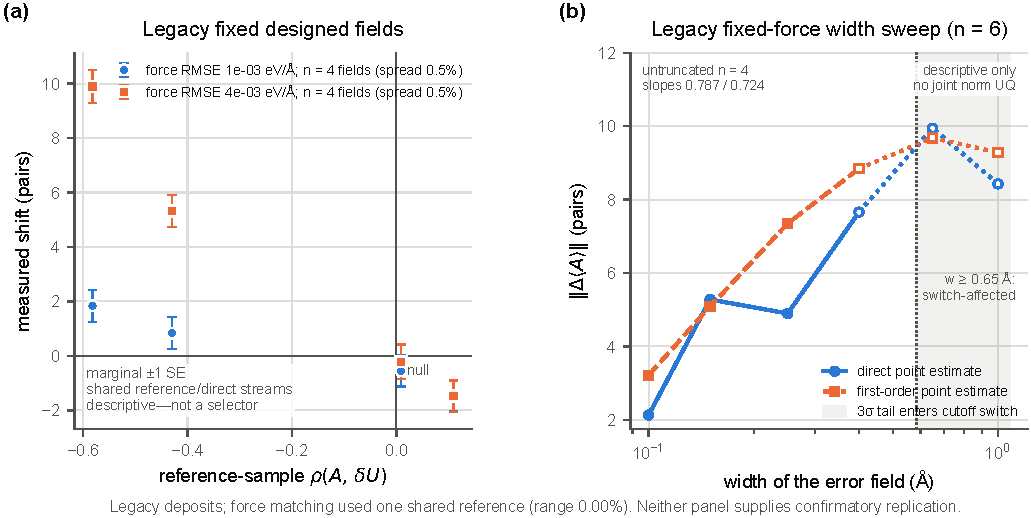
\includegraphics[width=6.6in]{headline_mechanism.pdf}
\caption{\label{fig:mechanism}%
The mechanism, at force RMSE held fixed in both panels.
(a) Measured shift in the target pair count (the bin from 3.4 to 3.9~\AA), in
pairs, against the Pearson correlation $\rho(A,\dU)$ between that observable and
the error field, for the four designed fields of
Table~\ref{tab:counterexamples} at out-of-sample force RMSE matched to 0.5\%.
The relation is monotone and close to linear, as
$\Delta\avg{A} = -\beta\,\sigma_0(A)\,\sigma_0(\dU)\,\rho_0(A,\dU)$ requires.
(b) Norm of the measured shift in the eight-bin difference curve, in pairs,
against the width $w$ of a Gaussian shell error field at
$r_0 = 4.2$~\AA, with the amplitude rescaled at each width so that the force
RMSE is $2.0\times10^{-3}~\eVA$ throughout; the residual spread in force RMSE
across the sweep is $3.3\times10^{-15}~\eVA$. The measured range is a factor of
4.66. Error bars are standard errors from Flyvbjerg--Petersen blocking; no
$1/\sqrt{M}$ estimate is used anywhere. The same width sweep appears in
Fig.~\ref{fig:response}(b) on logarithmic axes, where the exponent is fitted.}
\end{figure*}

\begin{figure}[t]
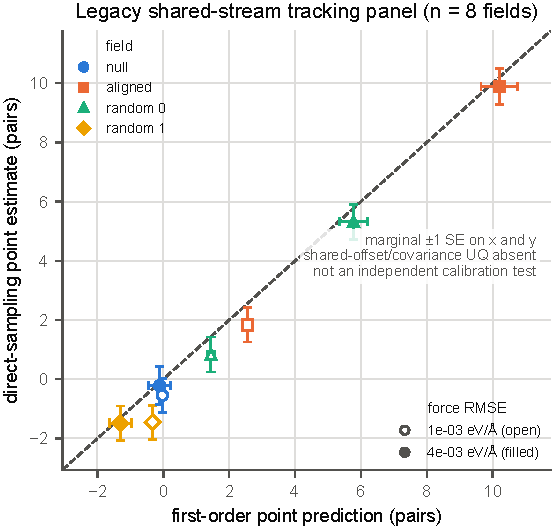
\includegraphics[width=3.3in]{headline_prediction.pdf}
\caption{\label{fig:prediction}%
Measured against predicted shift in the target pair count, in pairs, for all
eight designed error fields ($n = 8$; four fields at each of two force levels).
The prediction is $-\beta\,\Cov_0(A,\dU)$ evaluated on reference-ensemble
samples alone --- no molecular dynamics or Monte Carlo with any surrogate
entered it --- and the measurement comes from explicit Hamiltonian Monte Carlo
sampling of each perturbed potential. The line is the identity. The
root-mean-square residual, measured minus predicted in units of the standard
error of the measurement, is $1.01\sigma$. Error bars are standard errors.}
\end{figure}

\begin{figure*}[t]
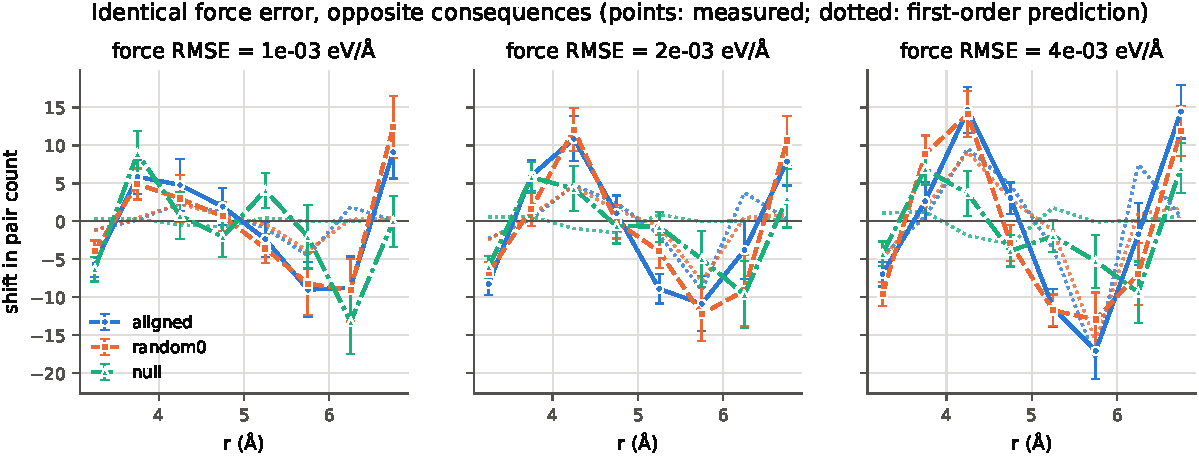
\includegraphics[width=6.6in]{exp07_designed_counterexamples_counterexamples.pdf}
\caption{\label{fig:counterexamples}%
Shift in pair count against pair separation $r$ for the null, aligned and random
error fields, one panel per force level ($1\times10^{-3}$ and
$4\times10^{-3}~\eVA$). The null field's target bin --- the one it was
constructed to be orthogonal to, from 3.4 to 3.9~\AA{} --- is left alone
($-0.220 \pm 0.640$ pairs at the upper level), but its largest non-target
excursion, $11.36 \pm 0.95$ pairs, is comparable to the aligned field's
$11.18 \pm 1.21$ pairs. Orthogonality is specific to the observable it was built
for. Error bars are standard errors from blocking.}
\end{figure*}

\begin{figure*}[t]
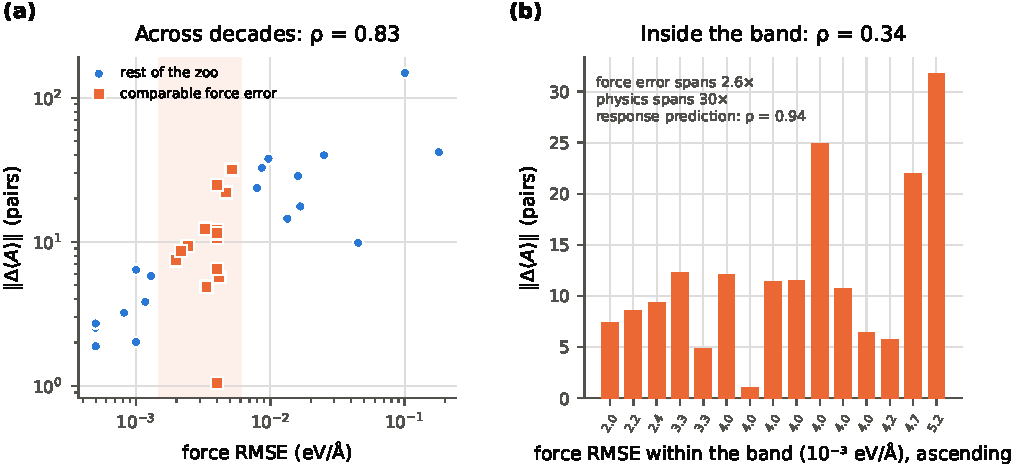
\includegraphics[width=6.6in]{headline_regimes.pdf}
\caption{\label{fig:regimes}%
Two regimes for force RMSE as a ranking metric, over the 34 designed surrogates.
(a) Observable error --- the noise-subtracted norm of the eight-bin difference
curve, in pairs --- against force RMSE on log--log axes, with the band
$1.5$--$6.0\times10^{-3}~\eVA$ shaded. Across the zoo the Spearman rank
correlation is $\rho = 0.83$ [0.67, 0.93], $n = 34$. (b) Observable error for
the 15 band members, ordered by ascending force RMSE: force RMSE spans a factor
of 2.59 while the observable error spans a factor of 30, giving
$\rho = 0.34$ [$-0.26$, 0.77], $n = 15$, an interval that includes zero, against
$\rho = 0.94$ [0.76, 1.00], $n = 15$ for the response prediction. \textbf{The
band is analyst-chosen and post hoc}: it was fixed after inspecting the data and
was not pre-registered. Intervals are 95\% percentile bootstrap over zoo
members. The panel titles in the published figure quote the point estimates
without intervals; the intervals are as given here.}
\end{figure*}

\begin{figure*}[t]
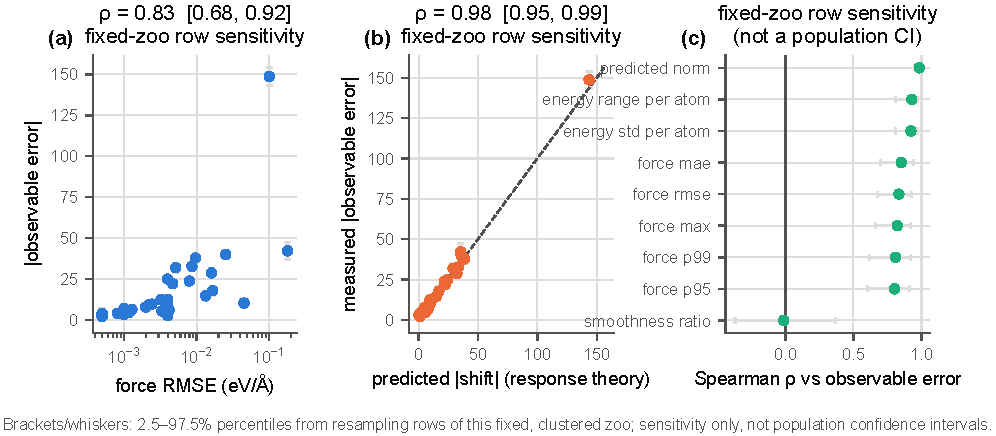
\includegraphics[width=6.6in]{exp05_proxy_correlation_proxy_correlation.pdf}
\caption{\label{fig:proxies}%
Proxy metrics against measured observable error across the 34 designed
surrogates. (a) Observable error against force RMSE, with standard-error bars;
the rank correlation for this panel is given in Fig.~\ref{fig:regimes}(a) and is
not restated here. (b) Measured against predicted observable error, the
prediction being the norm of $-\beta\,\Cov_0(A_k,\dU)$ from reference-ensemble
samples alone. (c) Spearman $\rho$ with 95\% bootstrap intervals for every proxy
metric. Panel (c) is where two results of Sec.~\ref{sec:regimes} are visible:
the smoothness ratio $\sigma_0(\dU)/\mathrm{RMSE}_F$, proposed in this work,
gives $\rho = -0.02$ [$-0.37$, 0.35], $n = 34$ and is refuted; the per-atom
energy spread gives $\rho = 0.92$ [0.82, 0.97], $n = 34$ and outranks every
force metric, which the theory does not predict.}
\end{figure*}

\begin{figure*}[t]
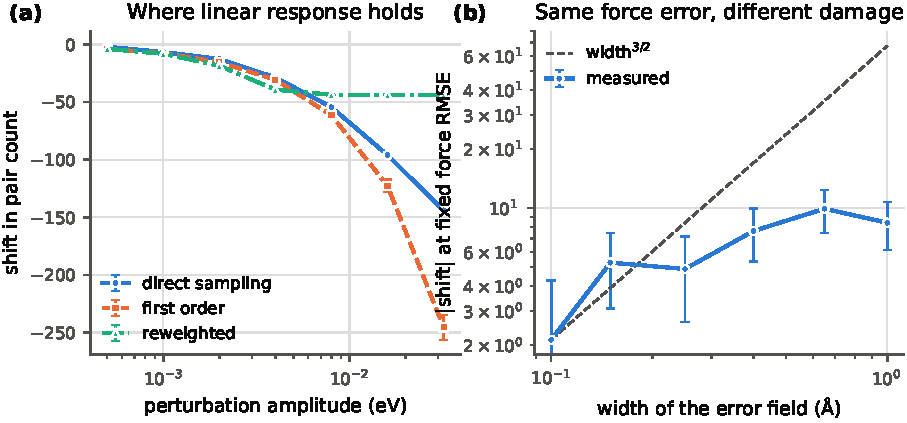
\includegraphics[width=6.6in]{exp06_response_validation_response_validation.pdf}
\caption{\label{fig:response}%
Validation and breakdown of the response estimators.
(a) First-order, exactly reweighted and directly sampled shifts in the peak bin,
in pairs, against the amplitude of a Gaussian shell perturbation at
$r_0 = 4.2$~\AA, $w = 0.35$~\AA. All three agree at amplitude
$1\times10^{-3}$ ($\beta\sigma_0(\dU) = 0.854$, the largest value at which they
do); above it the first-order estimate continues to grow linearly while the
direct measurement saturates and the reweighting estimate collapses as its
effective-sample-size fraction falls from 0.83 to $5\times10^{-4}$. The
disagreement at the \emph{smallest} amplitude is the unresolved discrepancy of
Sec.~\ref{sec:discrepancy}.
(b) Norm of the shift at fixed force RMSE against the width $w$ of the error
field, on log--log axes, from which the exponents are fitted: 0.56 from the
direct sampling and 0.45 from the first-order prediction, \textbf{against the
1.5 predicted in Sec.~\ref{sec:retraction}, which is thereby refuted}. This is
the same width sweep as Fig.~\ref{fig:mechanism}(b), where its dynamic range is
reported. Error bars are standard errors; where a plotted quantity is a fitted
exponent rather than a sampled mean, no error bar is drawn.}
\end{figure*}

%======================================================================
% TABLES
%======================================================================

% Source: results/exp07_designed_counterexamples/records.json
\begin{table*}[t]
\caption{\label{tab:counterexamples}%
Four designed error fields at two matched force-RMSE levels. $\rho(A,\dU)$ is
the Pearson correlation between the target observable (the pair count between
3.4 and 3.9~\AA) and the error field under the reference ensemble; the predicted
shift is $-\beta\,\Cov_0(A,\dU)$ from reference-ensemble samples alone; the
measured shift is from explicit Hamiltonian Monte Carlo sampling of the
perturbed potential. Force RMSE is quoted out of sample, on the half of the
reference trajectory not used to construct the fields; within each level the
four values agree to \textbf{0.5\%}. \textbf{Every $\pm$ in this table, and
everywhere in this article, is a standard error} --- from Flyvbjerg--Petersen
blocking for means and a moving-block bootstrap for covariances --- never a
standard deviation, and $1/\sqrt{M}$ is never used. The $\sigma$-distance is
$|\text{measured}|/|\text{its standard error}|$.}
\begin{ruledtabular}
\begin{tabular}{llccr@{\,$\pm$\,}lr@{\,$\pm$\,}lc}
Level & Field & RMSE$_F$ (out of sample, $\eVA$) & $\rho(A,\dU)$ &
\multicolumn{2}{c}{predicted (pairs)} & \multicolumn{2}{c}{measured (pairs)} &
$\sigma$ \\
\colrule
$1.0\times10^{-3}$ & null            & $1.00054\times10^{-3}$ & $+0.009$ & $-0.028$ & $0.083$ & $-0.547$ & $0.580$ & 0.9 \\
                   & random (seed 1) & $0.99896\times10^{-3}$ & $+0.110$ & $-0.327$ & $0.083$ & $-1.450$ & $0.576$ & 2.5 \\
                   & random (seed 0) & $0.99775\times10^{-3}$ & $-0.430$ & $+1.445$ & $0.104$ & $+0.835$ & $0.589$ & 1.4 \\
                   & aligned         & $0.99535\times10^{-3}$ & $-0.582$ & $+2.552$ & $0.140$ & $+1.835$ & $0.579$ & 3.2 \\
\colrule
$4.0\times10^{-3}$ & null            & $4.00217\times10^{-3}$ & $+0.009$ & $-0.113$ & $0.333$ & $-0.220$ & $0.640$ & 0.3 \\
                   & random (seed 1) & $3.99586\times10^{-3}$ & $+0.110$ & $-1.306$ & $0.331$ & $-1.482$ & $0.579$ & 2.6 \\
                   & random (seed 0) & $3.99100\times10^{-3}$ & $-0.430$ & $+5.778$ & $0.417$ & $+5.320$ & $0.589$ & 9.0 \\
                   & aligned         & $3.98141\times10^{-3}$ & $-0.582$ & $+10.206$ & $0.558$ & $+9.891$ & $0.611$ & 16.2 \\
\end{tabular}
\end{ruledtabular}
\end{table*}

% Source: results/exp07_designed_counterexamples/summary.json (null_space_generalisation)
%         and results/exp07_designed_counterexamples/generalisation.json
\begin{table}[t]
\caption{\label{tab:budget}%
How many frames the null-space construction needs. The field is built on
$n_{\rm construct}$ frames of the reference trajectory and evaluated on disjoint
frames. In sample the predicted shift is zero to machine precision by
construction; out of sample it is not, and the table shows that it remains small
from 250 frames upward. For scale, the aligned field at the same force error
($4\times10^{-3}~\eVA$) has a predicted shift of $10.206$ pairs, so the
suppression out of sample is roughly $400\times$. An earlier construction using
30 frames gave 1.2--1.6 pairs. $\pm$ is a standard error.}
\begin{ruledtabular}
\begin{tabular}{crr@{\,$\pm$\,}l}
$n_{\rm construct}$ & in sample (pairs) & \multicolumn{2}{c}{out of sample (pairs)} \\
\colrule
250  & $9.1\times10^{-15}$ & $0.041$ & $0.067$ \\
500  & $1.2\times10^{-15}$ & $0.142$ & $0.071$ \\
1000 & $5.0\times10^{-15}$ & $0.037$ & $0.077$ \\
2000 & $8.4\times10^{-15}$ & $0.028$ & $0.078$ \\
\end{tabular}
\end{ruledtabular}
\end{table}

% Source: results/exp05_proxy_correlation/{summary,records}.json and
%         scripts/compute_band_correlations.py (seed 20240517, 2000 resamples)
\begin{table}[t]
\caption{\label{tab:regimes}%
Two regimes, across the 34-member designed-surrogate zoo and within the band.
All correlations are Spearman rank correlations against the measured observable
error, computed on the noise-subtracted series (Sec.~\ref{sec:uncertainty}),
with 95\% percentile bootstrap intervals over zoo members from 2000 resamples,
seed 20240517. \textbf{The band --- force RMSE in
$1.5$--$6.0\times10^{-3}~\eVA$ --- is analyst-chosen and post hoc}, fixed after
inspecting the data and not pre-registered. The response prediction is the norm
of $-\beta\,\Cov_0(A_k,\dU)$. Footnote: on the raw (non-noise-subtracted) series
the zoo values are force RMSE $\rho = 0.83$ [0.68, 0.92], force MAE
$\rho = 0.85$ [0.70, 0.94], per-atom energy spread $\rho = 0.92$ [0.81, 0.97],
smoothness ratio $\rho = -0.01$ [$-0.37$, 0.37], response prediction
$\rho = 0.98$ [0.95, 0.99], all $n = 34$ with 2000 resamples; every value moves
by less than 0.01.}
\begin{ruledtabular}
\begin{tabular}{lcc}
 & across the zoo ($n = 34$) & within the band ($n = 15$) \\
\colrule
force-RMSE spread & $361\times$ & $2.59\times$ \\
observable-error spread & --- & $30\times$ \\
$\rho$(force RMSE) & 0.83 [0.67, 0.93] & 0.34 [$-0.26$, 0.77] \\
$\rho$(response prediction) & 0.98 [0.95, 0.99] & 0.94 [0.76, 1.00] \\
$\rho$(smoothness ratio) & $-0.02$ [$-0.37$, 0.35] & 0.84 [0.49, 0.98] \\
$\rho$(per-atom energy spread) & 0.92 [0.82, 0.97] & 0.91 [0.71, 0.99] \\
\end{tabular}
\end{ruledtabular}
\end{table}

% Source: results/exp03_model_zoo/records.json, summary.json
\begin{table*}[t]
\caption{\label{tab:zoo}%
The ten fitted models, all trained on 400 configurations of Lennard-Jones argon
with training and test data drawn from separate Markov chains. The predicted
shift is $-\beta\,\Cov_0(A,\dU)$ from reference-ensemble samples alone; the
measured shift is from direct sampling of each fitted model. The
root-mean-square prediction residual over the ten is $1.06\sigma$. \textbf{The
rank correlations from this arm are not reportable}: every interval spans zero
(force RMSE $\rho = 0.43$ [$-0.35$, 0.96], $n = 10$), because at this data
budget on this reference nearly every architecture is good enough that its
observable error is indistinguishable from zero. Nothing about ranking is
concluded from this arm. The two \texttt{egnn\_c8} rows differ only in
initialisation seed and are an illustration at \textbf{$n = 2$}, not a
statistic. The second-order ratio is the self-diagnostic of
Sec.~\ref{sec:cumulant}(iii); it flags 8 of 10 models as linearly trustworthy,
and the two it does not flag are the EGNN pair. $\pm$ is a standard error.}
\begin{ruledtabular}
\begin{tabular}{llcr@{\,$\pm$\,}lr@{\,$\pm$\,}lccc}
Model & Architecture & RMSE$_F$ ($\eVA$) &
\multicolumn{2}{c}{predicted (pairs)} & \multicolumn{2}{c}{measured (pairs)} &
$\sigma$ & 2nd-order ratio & trustworthy \\
\colrule
\texttt{spline\_k8}    & pair spline, 8 knots   & 0.00472 & $+1.667$ & $0.107$ & $+0.982$ & $0.564$ & 1.7 & 0.017 & yes \\
\texttt{spline\_k24}   & pair spline, 24 knots  & 0.00088 & $+0.245$ & $0.067$ & $+0.049$ & $0.603$ & 0.1 & 0.090 & yes \\
\texttt{linear\_l2}    & linear ACE-style, $l\le2$ & 0.00070 & $-0.044$ & $0.035$ & $-0.920$ & $0.549$ & 1.7 & 0.131 & yes \\
\texttt{linear\_l4}    & linear ACE-style, $l\le4$ & 0.00065 & $-0.064$ & $0.022$ & $-0.478$ & $0.611$ & 0.8 & 0.005 & yes \\
\texttt{bpnn\_16x2\_s0} & Behler--Parrinello, $16\times2$ & 0.00042 & $+0.250$ & $0.043$ & $-0.065$ & $0.631$ & 0.1 & 0.009 & yes \\
\texttt{bpnn\_16x2\_s1} & Behler--Parrinello, $16\times2$ & 0.00041 & $+0.257$ & $0.042$ & $-0.467$ & $0.580$ & 0.8 & 0.010 & yes \\
\texttt{bpnn\_64x2\_s0} & Behler--Parrinello, $64\times2$ & 0.00044 & $+0.236$ & $0.041$ & $+0.589$ & $0.620$ & 1.0 & 0.014 & yes \\
\texttt{bpnn\_64x2\_s1} & Behler--Parrinello, $64\times2$ & 0.00040 & $+0.235$ & $0.041$ & $+0.365$ & $0.564$ & 0.6 & 0.018 & yes \\
\texttt{egnn\_c8\_s0}  & $E(3)$-equivariant, seed 0 & 0.00450 & $-0.979$ & $0.206$ & $-0.152$ & $0.567$ & 0.3 & 0.412 & no \\
\texttt{egnn\_c8\_s1}  & $E(3)$-equivariant, seed 1 & 0.00609 & $-3.028$ & $0.290$ & $-4.101$ & $0.686$ & 6.0 & 0.142 & no \\
\end{tabular}
\end{ruledtabular}
\end{table*}

% Source: results/exp03_model_zoo_n400/records.json, summary.json
\begin{table}[t]
\caption{\label{tab:breakdown}%
The large-$\dU$ arm: four models fitted at a training budget of 20
configurations and run in the reduced quick-run mode, which puts them well
outside the perturbative regime. The aggregate root-mean-square prediction
residual is $30.4\sigma$, $n = 4$, against $1.01\sigma$ and $1.06\sigma$ in the
perturbative arms. \textbf{These records do not carry the
\texttt{second\_order\_ratio} or \texttt{linear\_trustworthy} fields, so the
second-order self-diagnostic cannot be checked against this arm}; that is a gap
in the evidence for the warning-light claim of Sec.~\ref{sec:cumulant}(iii).
$\pm$ is a standard error.}
\begin{ruledtabular}
\begin{tabular}{lcr@{\,$\pm$\,}lr@{\,$\pm$\,}lc}
Model & RMSE$_F$ ($\eVA$) & \multicolumn{2}{c}{predicted (pairs)} &
\multicolumn{2}{c}{measured (pairs)} & $\sigma$ \\
\colrule
\texttt{spline\_k12}    & $1.55\times10^{-3}$ & $+0.026$ & $0.251$ & $-5.173$ & $1.863$ & 2.8 \\
\texttt{linear\_l3}     & $5.08\times10^{-4}$ & $+0.180$ & $0.092$ & $-6.120$ & $2.438$ & 2.6 \\
\texttt{bpnn\_16x2\_s0} & $1.53\times10^{-2}$ & $-4.938$ & $2.297$ & $-14.507$ & $1.820$ & 5.3 \\
\texttt{egnn\_c8\_s0}   & $4.34\times10^{-2}$ & $-14.180$ & $7.337$ & $-126.160$ & $1.849$ & 60.5 \\
\colrule
\multicolumn{6}{l}{aggregate rms residual} & \textbf{30.4} \\
\end{tabular}
\end{ruledtabular}
\end{table}

% Source: results/exp06_response_validation/amplitude_records.json (rows 1-3)
%         and the recorded output of scripts/check_between_chain_scatter.py
\begin{table}[t]
\caption{\label{tab:discrepancy}%
The open discrepancy of Sec.~\ref{sec:discrepancy}. Upper block: three estimates
of the same shift at the smallest perturbation amplitude of the sweep, in the
peak bin at 4.25~\AA. The two estimators sharing the reference samples agree to
1.3\%; the direct estimate, which needs an independent chain, differs from both
by a factor of two. Lower block: the between-chain diagnostic, run on the same
perturbation but on the bin at 5.25~\AA, which overturns the obvious
explanation --- blocking is conservative here, not optimistic. \textbf{Three
explanations are excluded by measurement (error bars, second-order truncation,
incomplete relaxation) and the item is unresolved}; the remaining candidate, the
correlated-sample behaviour of the reweighting estimator's effective sample
size, was not tested. The lower block is the recorded output of the deposited
script \texttt{check\_between\_chain\_scatter.py} and is not written to a
\texttt{results/*.json} file. $\pm$ is a standard error.}
\begin{ruledtabular}
\begin{tabular}{lr}
Quantity & Value (pairs) \\
\colrule
\multicolumn{2}{l}{\emph{Peak bin, 4.25~\AA, amplitude $5\times10^{-4}$}} \\
first order & $-3.835 \pm 0.170$ \\
exact reweighting (ESS fraction 0.83) & $-3.884$ \\
direct sampling & $-1.948 \pm 0.821$ \\
\colrule
\multicolumn{2}{l}{\emph{Between-chain diagnostic, bin at 5.25~\AA, $n = 6$ seed pairs}} \\
within-chain blocking error & 0.589 \\
between-chain scatter & 0.312 \\
ratio (between/within) & 0.53 \\
six-seed mean shift & $+2.377 \pm 0.144$ \\
fresh-chain first order & $+1.725 \pm 0.101$ \\
fresh-chain exact reweighting & $+1.757$ \\
\end{tabular}
\end{ruledtabular}
\end{table}

% Source: docs/methods.md Sec. 1 / docs/validation.md Sec. 2
\begin{table}[t]
\caption{\label{tab:cutoff}%
Energy and force discontinuities of the four Lennard-Jones cutoff modes,
measured at $r_c \mp 10^{-7}$~\AA{} with $r_c = 7.0$~\AA. The
\texttt{shifted} mode, which is the common choice, removes the energy jump and
leaves the force jump untouched. \texttt{shifted\_force} is used throughout this
work.}
\begin{ruledtabular}
\begin{tabular}{lcc}
Mode & $|\Delta u|$ (eV) & $|\Delta F|$ ($\eVA$) \\
\colrule
\texttt{truncated}     & $2.4\times10^{-4}$  & $1.8\times10^{-4}$ \\
\texttt{shifted}       & $1.8\times10^{-11}$ & $1.8\times10^{-4}$ \\
\texttt{shifted\_force}& $8.7\times10^{-19}$ & $1.6\times10^{-11}$ \\
\texttt{switched}      & $2.2\times10^{-19}$ & $1.4\times10^{-16}$ \\
\end{tabular}
\end{ruledtabular}
\end{table}

% Source: docs/validation.md
\begin{table}[t]
\caption{\label{tab:validation}%
Validation against targets from outside the codebase. The Stillinger--Weber
entry is an \emph{exactness check} and carries its full digits for that reason:
at the diamond lattice constant the answer is $-2\epsilon$ identically. The
embedded-atom copper entry is the one worth dwelling on --- the potential
reproduces its three fitted targets exactly and still gives a maximum phonon
frequency about 30\% below copper's, which is the statement this paper makes
about force error arriving from a different direction. $\pm$ is a standard
error.}
\begin{ruledtabular}
\begin{tabular}{lll}
Check & Target & Obtained \\
\colrule
SW Si cohesive energy & exactly $-2\epsilon = -4.33660$~eV/atom & $-4.3366000$ \\
LJ fcc lattice sum & $-8.6108\,\epsilon$/atom & $-8.603$ (cutoff-extrapolated) \\
EAM Cu lattice constant & 3.615~\AA & 3.6150~\AA \\
EAM Cu cohesive energy & $-3.54$~eV/atom & $-3.5400$~eV/atom \\
EAM Cu bulk modulus & 140~GPa & 140.0~GPa \\
EAM Cu max.\ phonon freq. & $\approx 7.5$~THz (real Cu) & 5.14~THz \\
fcc/bcc/sc $Q_6$ & 0.5745 / 0.5106 / 0.3536 & 0.5745 / 0.5107 / 0.3536 \\
SOAP rotational invariance & 0 & $8\times10^{-15}$ \\
ACSF rotational invariance & 0 & $2\times10^{-15}$ \\
HMC $\avg{U}$ (Einstein crystal) & 0.41363~eV & $0.41462 \pm 0.00196$ ($0.5\sigma$) \\
HMC $\Var(U)$ (Einstein crystal) & 0.003564~eV$^2$ & 0.003459~eV$^2$ \\
Phonon dispersion & $2\sqrt{k/m}\,|\sin(qa/2)|$ & $10^{-5}$ relative \\
\end{tabular}
\end{ruledtabular}
\end{table}

\bibliographystyle{aipnum4-2}
\bibliography{refs}

\end{document}
